% Condensed edition: main findings, the model and its proofs, the ledger of
% departures, and the experiment results. Built from the same section files
% as main.tex (the extended edition). References with an F-numbered target
% resolve through build/labels-from-full.tex, generated from the extended
% edition's .aux by tools/make-label-shim.py, and point into that edition.
\documentclass[11pt,a4paper]{article}

% Preamble: packages, theorem environments, and page furniture.

\usepackage[T1]{fontenc}
\usepackage{lmodern}
\usepackage{microtype}

\usepackage[a4paper,margin=27mm]{geometry}
\usepackage{ragged2e}
\usepackage{amsmath}
\usepackage{amssymb}
\usepackage{amsthm}
\usepackage{booktabs}
\usepackage{longtable}
\usepackage{array}
\usepackage{enumitem}
\usepackage{verbatim}
\usepackage{xcolor}
\usepackage{fancyvrb}
\usepackage{tikz}
\usetikzlibrary{arrows.meta,positioning}

% Identifiers and paths set in \texttt are the only things in this document
% long enough to overflow a line; htt lets TeX hyphenate them, and the
% emergency stretch absorbs what is left.
\usepackage[htt]{hyphenat}
\setlength{\emergencystretch}{2.5em}

\usepackage[hidelinks]{hyperref}
\usepackage[capitalise,noabbrev]{cleveref}

% One shared counter for every numbered result, so a reference to "Theorem 12"
% can never collide with "Lemma 12" and the reader can find any of them by
% counting forwards.
\theoremstyle{plain}
\newtheorem{theorem}{Theorem}
\newtheorem{lemma}[theorem]{Lemma}
\newtheorem{proposition}[theorem]{Proposition}
\newtheorem{corollary}[theorem]{Corollary}

\theoremstyle{definition}
\newtheorem{definition}[theorem]{Definition}
\newtheorem{example}[theorem]{Example}
\newtheorem{obligation}[theorem]{Proof obligation}

\theoremstyle{remark}
\newtheorem{remark}[theorem]{Remark}

\crefname{obligation}{proof obligation}{proof obligations}
\Crefname{obligation}{Proof obligation}{Proof obligations}

% Pseudocode transcribed from the specification. Kept verbatim rather than
% reset in a pretty algorithm environment: the whole point is that the reader
% can diff it against SPEC.md by eye.
\DefineVerbatimEnvironment{speccode}{Verbatim}%
  {fontsize=\small,frame=leftline,framerule=0.6pt,%
   xleftmargin=10pt,framesep=8pt}

% Table columns hold package names, test identifiers and other unbreakable
% strings; ragged right is the only setting under which they do not overflow.
\newcolumntype{L}[1]{>{\RaggedRight\arraybackslash}p{#1}}

\setlist{itemsep=2pt,topsep=4pt,parsep=0pt}
\setlength{\parskip}{0.4em}
\setlength{\parindent}{0pt}

\hypersetup{
  pdftitle={The CCME release guarantees: a formal model and proofs},
  pdfsubject={Formal properties of the Conventional Commits Monorepo Extension release algorithm},
  pdfkeywords={release engineering, monorepo, semantic versioning, convergence, distributed transactions}
}

% One macro per notion of the specification. Nothing in this document types a
% symbol directly: if a definition changes, it changes here, and the appendix
% symbol table is written from this file.

% ---- cross-references into the sources -------------------------------------
% \textup so that small caps survive the italic body of a theorem environment,
% where T1/lmr/m/scit does not exist.
\newcommand{\SPEC}{\textup{\textsc{spec}}}
\newcommand{\spec}[1]{\SPEC~\S#1}
\newcommand{\specs}[2]{\SPEC~\S\S#1,~#2}
\newcommand{\code}[1]{\texttt{#1}}
\newcommand{\diag}[1]{\texttt{#1}}          % a diagnostic code, e.g. \diag{W208}

% ---- history ---------------------------------------------------------------
\newcommand{\Cmts}{\ensuremath{\mathcal{K}}}            % the set of commits
\newcommand{\Head}{\ensuremath{h}}                      % HEAD, fixed throughout
\newcommand{\Rch}[1]{\ensuremath{\mathrm{reach}(#1)}}   % ancestors-or-self
\newcommand{\anc}{\ensuremath{\preceq}}                 % ancestor-or-self

% ---- workspace -------------------------------------------------------------
\newcommand{\Pkgs}{\ensuremath{\mathcal{P}}}            % packages at HEAD
\newcommand{\Edges}{\ensuremath{E}}                     % dependency edges
\newcommand{\Dep}[1]{\ensuremath{\mathrm{dep}(#1)}}     % direct dependents of a package
\newcommand{\dist}[2]{\ensuremath{\delta(#1,#2)}}       % shortest edge count, set to package
\newcommand{\reachset}[2]{\ensuremath{R(#1,#2)}}        % the traversal of §9.2

% ---- bumps and versions ----------------------------------------------------
\newcommand{\Bumps}{\ensuremath{\mathbb{B}}}
\newcommand{\bnone}{\ensuremath{\mathsf{none}}}
\newcommand{\bpatch}{\ensuremath{\mathsf{patch}}}
\newcommand{\bminor}{\ensuremath{\mathsf{minor}}}
\newcommand{\bmajor}{\ensuremath{\mathsf{major}}}
\newcommand{\Vers}{\ensuremath{\mathcal{V}}}
\newcommand{\applyb}[2]{\ensuremath{\mathrm{apply}(#1,#2)}}
\newcommand{\coreof}[1]{\ensuremath{\mathrm{core}(#1)}}
\newcommand{\cntof}[1]{\ensuremath{\mathrm{cnt}(#1)}}

% ---- channels --------------------------------------------------------------
\newcommand{\Chans}{\ensuremath{\mathcal{C}\!h}}
\newcommand{\stable}{\ensuremath{\mathsf{stable}}}
\newcommand{\chanof}[1]{\ensuremath{\mathrm{ch}(#1)}}   % the channel of a version
\newcommand{\NONE}{\ensuremath{\bot}}                   % "proposes nothing"

% ---- state and its derived quantities --------------------------------------
\newcommand{\st}{\ensuremath{\sigma}}
\newcommand{\Win}[2]{\ensuremath{W_{#1}(#2)}}                  % train window
\newcommand{\Winf}[2]{\ensuremath{W^{\circ}_{#1}(#2)}}         % undelivered admission window
\newcommand{\base}[2]{\ensuremath{\mathrm{base}_{#1}(#2)}}
\newcommand{\basec}[2]{\ensuremath{\mathrm{basec}_{#1}(#2)}}   % commit of the baseline tag
\newcommand{\stbase}[2]{\ensuremath{\mathrm{sbase}_{#1}(#2)}}
\newcommand{\stcommit}[2]{\ensuremath{\mathrm{scom}_{#1}(#2)}}
\newcommand{\chanres}[2]{\ensuremath{\mathrm{chan}_{#1}(#2)}}  % channel(P), §13.8

% ---- units and their directives --------------------------------------------
\newcommand{\Units}{\ensuremath{\mathcal{U}}}
\newcommand{\cof}[1]{\ensuremath{c_{#1}}}                      % the commit carrying a unit
\newcommand{\scopef}[1]{\ensuremath{\mathrm{scope}(#1)}}
\newcommand{\bumpof}[1]{\ensuremath{\mathrm{bump}(#1)}}
\newcommand{\pbump}[1]{\ensuremath{\mathrm{pb}(#1)}}           % effective propagated bump
\newcommand{\pdepth}[1]{\ensuremath{\mathrm{pd}(#1)}}
\newcommand{\pscope}[1]{\ensuremath{\mathrm{ps}(#1)}}
\newcommand{\pchan}[1]{\ensuremath{\mathrm{pc}(#1)}}
\newcommand{\pcdepth}[1]{\ensuremath{\mathrm{pcd}(#1)}}
\newcommand{\pcscope}[1]{\ensuremath{\mathrm{pcs}(#1)}}

% ---- suppression, sources, admission ---------------------------------------
\newcommand{\disch}[3]{\ensuremath{\mathrm{disch}_{#1}(#2,#3)}}
\newcommand{\canc}[2]{\ensuremath{\mathrm{canc}(#1,#2)}}
\newcommand{\held}[1]{\ensuremath{\mathrm{held}(#1)}}
\newcommand{\srcp}[2]{\ensuremath{\mathrm{src}_{#1}(#2)}}
\newcommand{\srcch}[2]{\ensuremath{\mathrm{sch}_{#1}(#2)}}     % the source channel set, §9.3a
\newcommand{\resolv}[3]{\ensuremath{\mathrm{rsv}_{#1}(#2,#3)}}
\newcommand{\admit}[3]{\ensuremath{\mathrm{adm}_{#1}(#2,#3)}}

% ---- the plan --------------------------------------------------------------
\newcommand{\dirb}[2]{\ensuremath{\mathrm{dir}_{#1}(#2)}}
\newcommand{\propb}[2]{\ensuremath{\mathrm{prp}_{#1}(#2)}}
\newcommand{\effb}[2]{\ensuremath{\mathrm{eff}_{#1}(#2)}}
\newcommand{\plan}[1]{\ensuremath{\Pi(#1)}}
\newcommand{\vers}[2]{\ensuremath{\nu_{#1}(#2)}}
\newcommand{\Run}[2]{\ensuremath{\mathrm{run}(#1,#2)}}

% ---- guarantee labels ------------------------------------------------------
\newcommand{\G}[1]{\textbf{G#1}}

% ---- delivery (SPEC 13.3, 13.4a, 19.3; added for the 3.1.0-rc.2 text) ------
\newcommand{\relc}[2]{\ensuremath{T_{#1}(#2)}}                        % release commits of a package
\newcommand{\deliv}[4]{\ensuremath{\mathrm{dlv}_{#1}(#2,#3,#4)}}       % delivered(P, C, D)
\newcommand{\owed}[3]{\ensuremath{\mathrm{owed}_{#1}(#2,#3)}}          % owed(u, D)
\newcommand{\Wowed}[3]{\ensuremath{W^{\mathrm{ow}}_{#1}(#2,#3)}}       % owedWindow(P, D)
\newcommand{\owes}[3]{\ensuremath{\mathrm{owes}_{#1}(#2,#3)}}          % P still owes D
\newcommand{\owncause}[3]{\ensuremath{\mathrm{own}_{#1}(#2,#3)}}       % a cause of its own, §19.3
\newcommand{\wf}[1]{\ensuremath{\mathrm{wf}(#1)}}                      % E201 well-formedness of a state
\newcommand{\pubset}[2]{\ensuremath{S(#1,#2)}}                         % the packages a run publishes
\newcommand{\blocked}[2]{\ensuremath{B(#1,#2)}}                        % the packages a run blocks
\newcommand{\stale}[2]{\ensuremath{\mathrm{stale}_{#1}(#2)}}           % the upward audit, §13.7b
\newcommand{\Kprop}{\ensuremath{K_{\mathrm{prop}}}}                    % propagation.kinds
\newcommand{\Korder}{\ensuremath{K_{\mathrm{order}}}}                  % publish.orderKinds
\newcommand{\Kblock}{\ensuremath{K_{\mathrm{block}}}}                  % publish.blockingKinds

% ---- execution section (moved from sections/04a-execution.tex) --------------
% Symbols of the execution section, prefixed \ex.
\newcommand{\exafter}[2]{\ensuremath{A_{#1}(#2)}}          % after-set in repository #1 of boundary #2
\newcommand{\exRch}[2]{\ensuremath{\mathrm{reach}_{#1}(#2)}} % reachability inside one repository
\newcommand{\exWin}[2]{\ensuremath{W(#1;\,#2)}}             % train window of consumer #1 over repository #2
\newcommand{\exWinf}[2]{\ensuremath{W^{\circ}(#1;\,#2)}}    % fresh window of consumer #1 over repository #2
\newcommand{\exPlan}{\ensuremath{\mathrm{Plan}}}            % the pure planning function of §28.3
\newcommand{\exI}{\ensuremath{\mathcal{I}}}                 % the fixed run input of §28.3
\newcommand{\exbuild}[1]{\ensuremath{\mathrm{build}(#1)}}
\newcommand{\expub}[1]{\ensuremath{\mathrm{publish}(#1)}}

% ---- evaluation section (moved from sections/11-evaluation.tex) -------------
% \evpath sets a file path in monospace and lets it break after / . _ and -,
% through the url package that hyperref already loads. \evhash lets a hex
% digest break anywhere, since nothing in it is a word.
\DeclareUrlCommand\evpath{\urlstyle{tt}\def\UrlBreaks{\do\/\do\.\do\_\do\-\do\@\do\:}}
\newcommand{\evRQ}[1]{\textbf{RQ#1}}
\makeatletter
\newcommand{\evhash}[1]{\texttt{\ev@split#1\@nil}}
\def\ev@split#1#2\@nil{#1\ifx\relax#2\relax\expandafter\@gobble\else\expandafter\@firstofone\fi{\allowbreak\ev@split#2\@nil}}
\makeatother

\input{build/labels-from-full}

\title{The CCME Release Guarantees\\[2mm]
       \large Main findings, proofs and experimental results (condensed edition)}
\author{Semen Fediukovich}
\date{September 2026 \\[2mm]
      \normalsize Technical report accompanying \texttt{specs/ccme-spec/SPEC.md} 3.1.0-rc.2\\
      \normalsize at commit \texttt{252216ba} of \texttt{github.com/yohimik/dispat}}

\begin{document}
\maketitle

\begin{abstract}
Releasing interdependent packages is a distributed transaction without a
coordinator or rollback: each publish is an irreversible write to an
independent registry. CCME defines a resumable release algorithm and states
eight guarantees: termination, completeness, version stability, exactly-once
tag-ledger delivery, retry-invariant non-widening and convergence, channel
discharge and one-way axis independence.

This report formalises the algorithm of the 3.1.0 release candidate and proves
the guarantees under its explicit retry invariant. The candidate replaces the
window test of earlier versions by delivery: a propagated contribution stays
owed to a consumer until the source has released it and the consumer has
released after that, which closes the orphan a consumer reaches by getting
ahead of a failed provider, at the price of an owed window per dependency edge
and a refusal (\diag{E201}) where two releases on one commit could hide a debt.
The report also proves the determinism and idempotency requirements of
\spec{17.2} and the duality of \spec{13.7b}, and states what the build
readiness relation of \spec{19.2a} buys in run duration.

The current departures of the reference implementation from the candidate are
tabulated with their status. The final section reports every executed
campaign with its pinned binary and environment, including the two
measurements of 22 September 2026 on which the execution profile rests: two
kernel farm groups that met their public reference times with a second node,
twice each after one rejected candidate, and an LLVM matrix released through
two workers in less time than on one node, once per side, with a reproduction
kit whose binary rebuilds were verified byte for byte and whose machine
definitions were planned but not applied. The extended edition, built from
the same sources, adds the transcriptions of the distributed and
polyrepository profiles, the cost analysis, the historical audit of
CCME 1.0.0, the conformance table and the full campaign narratives.
\end{abstract}

\paragraph{Specification snapshot.}
The normative subject is \texttt{specs/ccme-spec/SPEC.md} as committed at
\texttt{252216bab9bd4052ba181a2ceb47e21363b8eff3}, stamped 3.1.0-rc.2 and
pending release as 3.1.0-rc.3 together with dispat 1.11.0-rc.4; its
\texttt{DESIGN-HISTORY.md} entries of 21 and 22 September 2026 record what the
engine implements. Where the report says \emph{the current text} it means this
commit; the released CCME 2.0.0 at \texttt{d3ce8ae6} is cited where a change
since then matters. A reference whose number carries an F, such as
Proposition~F73, points into the extended edition
(\texttt{technical-report-extended.pdf}).\par

\tableofcontents
\newpage

\section{Main findings}
\label{sec:intro}

\subsection{The problem}

A workspace is a repository holding many independently versioned packages that
depend on one another. Releasing it means choosing a new version for each
package that needs one, writing those versions into manifests, uploading
artefacts to registries, and recording what happened. The recording is the
hard part: registries have no transactions, a publish is an irreversible write
to a service the release tool does not control, several registries may be
involved, and no coordinator can commit or abort them as a unit. A run that
publishes seven packages is seven independent, individually fallible writes.

CCME\footnote{\emph{Conventional Commits: Monorepo Extension}, version
3.1.0-rc.2 at commit \texttt{252216ba}, \code{specs/ccme-spec/SPEC.md} in the
\code{dispat} repository. Referred to throughout as \SPEC{}, cited by section
number.} answers this the way a saga does. The release plan is a pure function
of the repository at a fixed commit; each completed leg is recorded by an
annotated git tag written immediately after that leg succeeds; and recovery is
re-execution: run the engine again and it recomputes the same transaction,
skipping the legs already recorded. That design works only if re-execution is
well behaved, and \spec{13.7c} states the eight properties that say it is:

\begin{description}[leftmargin=3.2em,style=nextline,font=\normalfont\bfseries]
  \item[\G{1} termination] propagation halts, whatever the declared depth.
  \item[\G{2} completeness] a contribution admitted to a dependent survives in
    every later run until that dependent releases at or after a release of
    every owed source carrying it; there are no orphans, whether the provider
    failed or the consumer got ahead of it.
  \item[\G{3} version stability] a package released late is released at the
    version it was originally planned at.
  \item[\G{4} no double ledger delivery] a contribution does not survive its
    delivery in the tag ledger; this says nothing unconditional about external
    effects.
  \item[\G{5} no blast-radius widening] under the retry invariant, later
    targets are a subset of the first run's.
  \item[\G{6} restricted convergence] under the retry invariant, repeated
    successful progress empties the initial plan within as many runs as it had
    publishable packages.
  \item[\G{7} channel discharge] a prerelease channel is proposed to a package
    only until it is released on it.
  \item[\G{8} one-way axis independence] suppressing a version bump does not
    suppress a channel change; resolved channels may suppress bumps.
\end{description}

\subsection{What this report establishes}

The report writes the algorithm down once, formally
(\cref{sec:model,sec:propagation,sec:protocol}), proves the guarantees inside
that model (\cref{sec:guarantees}), and reports what the reference
implementation was observed to do in the campaigns that were executed
(\cref{sec:evaluation}). The findings, each with the result that carries it:

\begin{enumerate}[leftmargin=2em]
  \item \textbf{The eight guarantees hold for the model under the explicit
    retry invariant of \spec{13.7c} and two hypotheses the specification does
    not state}, (R) that owed sources reach their target and (K) that
    propagation edges order and block (\cref{thm:g1,thm:g2,thm:g3,thm:g4,thm:g5,thm:g6,thm:g7,thm:g8}).
    (R) holds outright for a unit with a single source; it can fail for a
    multi-source unit, and the reference engine exhibited exactly that failure
    until a fix that postdates the measured builds (\cref{ob:attribution}).
  \item \textbf{Delivery closes the orphan a consumer reaches by getting ahead
    of a failed provider.} The candidate admits a propagated contribution
    until its source has delivered it (\spec{13.4a}); the model transcribes
    this test (\cref{def:delivery}) and \cref{thm:g2} is proved for it. Two
    rules follow and are stated as boundaries rather than proved away: an owed
    window per dependency edge and the refusal \diag{E201}, which the
    specification states and the engine does not yet implement
    (\cref{ob:owed}), and the same-commit case that the protocol reports
    rather than resolves (\cref{ob:samecommit}).
  \item \textbf{The plan is a deterministic, idempotent function of the fixed
    inputs, and a run after a partial failure plans the failed packages, the
    blocked ones and the consumers still owed} (\cref{thm:determinism},
    \cref{cor:idempotency}, \cref{thm:resumption}).
  \item \textbf{The staleness audit of \spec{13.7b} never over-reports and
    under-reports in three shapes}, all with a multi-source unit; the second
    shape is the engine defect above (\cref{thm:duality}, \cref{rem:owed-reach}).
  \item \textbf{Build readiness buys wall time in a form that can be stated.}
    With unlimited slots a run lasts its longest path and a weaker relation
    never lengthens it; the chain, fan-out and fan-in formulas are exact; under
    slot budgets a greedy schedule is within the list-scheduling bound and can
    show Graham's anomaly (\cref{sec:exec-durations}). The placement invariance
    of the distributed profile, that worker count, placement and completion
    order do not change the plan, is stated and proved in the extended edition
    (\cref{prop:exec-placement}).
  \item \textbf{The implementation departs from the text in eight recorded
    places}, none of which loses a release silently except the stranded
    consumer of \cref{ob:owed}; \cref{sec:departures} tabulates them with
    their status.
  \item \textbf{The measurements.} In every state of a finite projection and in
    every completed episode, the consumer-relative window retained exactly the
    residual obligations, and a source-relative window would have lost
    obligations in 84 of the 120 designed fault episodes and in 260 of 772
    states (\cref{sec:eval:rq1}). Recorded progress survived repeated failure
    without version drift in 130 of 130 rows, and the restricted oracle agreed
    on all 300 histories of each companion campaign (\cref{sec:eval:rq2}). A
    configured barrier distinguished local build availability from required
    publication, and both a failed and an absent required test blocked release
    (\cref{sec:eval:rq3}). Planning cost rose from 0.017~s at 100 packages to
    about 19~s at 10,000 on a capped host (\cref{sec:eval:rq4}). On a kernel
    build farm, two groups met their public reference times with a second node,
    twice each after one rejected candidate, where the same node alone did
    not; on an LLVM matrix, a release through two workers took 27:48.94
    against 41:12.02 on one node, once per side; a one-heavy-package fixture
    showed the predicted negative case (\cref{sec:eval:rq5}). No speedup of the
    profile or of the engine is claimed beyond what these pairs measured.
\end{enumerate}

\subsection{Scope, and how to read this edition}

The subject is the release computation of \spec{13} and the publish protocol
of \spec{19}, with the execution rules of \specs{19.2a}{28} as transcribed
obligations. Message syntax (\spec{4}--\spec{8}) is taken as given: units
arrive already parsed. Outside the theorems, and not spoken for by them, are
manifest range reconciliation (\spec{9.4}, \spec{19.5}), the diagnostic
registry of \spec{16} beyond the codes used as labels, executor scheduling
beyond the stated relations and bounds, shared-version groups
(\spec{13.9a}), and the adapter and rollback protocols of \specs{25}{26}. The
report claims no novelty for sagas, idempotent consumers, breadth-first
search or list scheduling; its contribution is the formal model, corrected
hypotheses, counterexamples, the ledger of departures, and the record of what
was measured.

This is the condensed edition. The extended edition, distributed beside it as
\code{technical-report-extended.pdf} and built from the same sources, adds the
transcriptions of the distributed profile (\spec{28}) and of the
repository-local windows (\spec{27}), the cost analysis of
\specs{13.11}{20.7}, the historical audit of CCME 1.0.0 with its six
counterexamples, the conformance table that maps every result to the
specification's vectors and to the integration test behind it, and the full
narratives of the campaigns, including every discarded attempt. A reference
whose number carries an F, such as \emph{Proposition F73}, points into the
extended edition; every other reference is to this document.
\Cref{appendix:notation} is the symbol table, and \cref{appendix:abstract}
reads the companion conference abstract against this report sentence by
sentence. \SPEC{} is licensed GPL-3.0-or-later and this report reproduces its
definitions and pseudocode; it is distributed under the same licence
(\code{paper/LICENSE}).

\section{The model}
\label{sec:model}

Everything in this report is stated over the objects defined here. Each
definition transcribes a numbered section of \SPEC{} and cites it. Where
the transcription makes a choice the source leaves implicit, the choice is
flagged in a remark rather than buried.

\subsection{History}

\begin{definition}[commit history, \spec{12.2}]
\label{def:history}
The history is a finite directed acyclic graph on a set of commits \Cmts, with
an edge from a commit to each of its parents. A distinguished commit
$\Head \in \Cmts$ is \emph{HEAD}. For $c \in \Cmts$,
$\Rch{c} \subseteq \Cmts$ is the set of commits reachable from $c$ by following
parent edges, including $c$ itself. Write $c' \anc c$ for $c' \in \Rch{c}$
(``$c'$ is an ancestor-or-self of $c$'').
\end{definition}

\Head{} is fixed for the whole report. The retry and convergence guarantees of \spec{13.7c} are stated at a fixed \Head{}; advancing it may legitimately add, remove, or redirect work. Structural termination and single-state determinism do not need that restriction.

\begin{remark}
Ancestry, not commit date or log order, is the only ordering used. This is what
makes cancellation deterministic under merges and rebases (\spec{10.4}) and
what lets the model ignore clocks entirely.
\end{remark}

\subsection{Workspace}

\begin{definition}[workspace graph, \spec{13.1}, \spec{8.4}]
\label{def:graph}
\Pkgs{} is the finite set of packages present at \Head{}. For a fixed set of
edge kinds $K$ (the configured \code{propagation.kinds}), $\Edges \subseteq
\Pkgs \times \Pkgs$ contains $(a,b)$ when $a$ declares a dependency on $b$ of a
kind in $K$. The \emph{dependents} of $p$ are $\Dep{p} = \{d : (d,p) \in
\Edges\}$. The graph $(\Pkgs, \Edges)$ is acyclic.
\end{definition}

Acyclicity is an assumption the model may make because the engine enforces it:
a cycle over the propagation or publish-ordering kinds is the repository-scoped
error \diag{E200} and aborts the run before any plan is computed. \spec{13.1}
justifies rejecting rather than accommodating cycles: no publish order exists
for a cycle, so whichever member goes first declares a range on a version that
does not yet exist, and if the run then fails that state is permanent.

Propagation travels \emph{against} the dependency edges, from a changed package
to the packages that consume it; that is, along \Dep{\cdot}.

\begin{example}[the running workspace, \spec{22}]
\label{ex:workspace}
The running examples use the six-package workspace shared by many conformance vectors:
\[
  \Pkgs = \{\,\code{core},\ \code{cli},\ \code{ui},\ \code{api},\
            \code{docs-site},\ \code{@acme/theme}\,\},
\]
\[
  \Edges = \{\,(\code{cli},\code{core}),\ (\code{ui},\code{core}),\
              (\code{api},\code{core}),\ (\code{docs-site},\code{ui}),\
              (\code{@acme/theme},\code{ui})\,\},
\]
drawn in \cref{fig:workspace}, with the initial tag state
\[
  \st_0 = \{\ \code{core@1.4.2},\ \code{cli@2.0.0},\ \code{ui@0.9.1},\
              \code{api@1.2.0},\ \code{@acme/theme@1.0.0}\ \}.
\]
\code{docs-site} has never been released, so it has no baseline; it is private
and publishes to an internal registry, which by \spec{13.10a} exempts it from
nothing.
\end{example}

\begin{figure}[t]
\centering
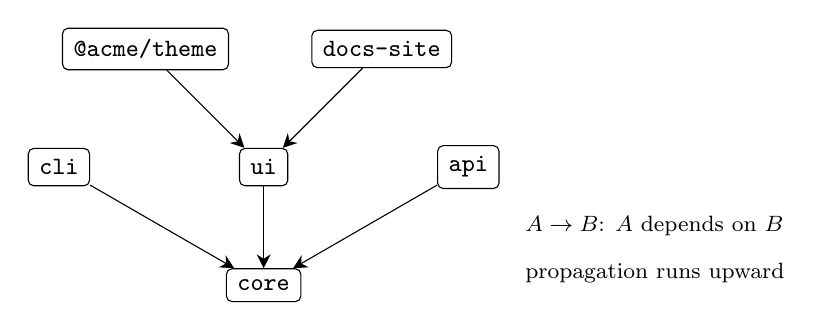
\begin{tikzpicture}[
    >={Stealth[width=5pt,length=5pt]},
    pkg/.style={draw,rounded corners=2pt,inner sep=4pt,font=\small\ttfamily},
    every edge/.style={draw,->}]
  \node[pkg] (core) at (0,0) {core};
  \node[pkg] (cli)  at (-2.6,1.5) {cli};
  \node[pkg] (ui)   at (0,1.5)    {ui};
  \node[pkg] (api)  at (2.6,1.5)  {api};
  \node[pkg] (theme) at (-1.5,3.0) {@acme/theme};
  \node[pkg] (docs)  at (1.5,3.0)  {docs-site};
  \draw[->] (cli)   -- (core);
  \draw[->] (ui)    -- (core);
  \draw[->] (api)   -- (core);
  \draw[->] (theme) -- (ui);
  \draw[->] (docs)  -- (ui);
  \node[font=\footnotesize,anchor=west] at (3.2,0.75)
    {$A \rightarrow B$: $A$ depends on $B$};
  \node[font=\footnotesize,anchor=west] at (3.2,0.15)
    {propagation runs upward};
\end{tikzpicture}
\caption{The running workspace of \cref{ex:workspace}. Distances from
$S=\{\code{core}\}$ are $\dist{S}{\code{cli}} = \dist{S}{\code{ui}} =
\dist{S}{\code{api}} = 1$ and $\dist{S}{\code{docs-site}} =
\dist{S}{\code{@acme/theme}} = 2$.}
\label{fig:workspace}
\end{figure}

\begin{definition}[distance, \spec{9.2}]
\label{def:dist}
For $S \subseteq \Pkgs$ and $d \in \Pkgs$, $\dist{S}{d}$ is the least $n$ for
which there are $p_0 \in S$ and $p_1,\dots,p_n = d$ with $p_{i+1} \in
\Dep{p_i}$ for all $i$, and $\infty$ if no such chain exists. Note
$\dist{S}{d} = 0$ exactly when $d \in S$.
\end{definition}

\subsection{Bumps and versions}

\begin{definition}[bumps, \spec{7.1}, \spec{9.1}]
\label{def:bump}
$\Bumps = \{\bnone, \bpatch, \bminor, \bmajor\}$ ordered
$\bnone < \bpatch < \bminor < \bmajor$. Being a finite chain, $(\Bumps, \leq)$
is a join-semilattice with least element \bnone{} and join $\sqcup = \max$.
\end{definition}

The whole of \spec{9.1}'s ``bumps accumulate'' is the statement that the
combining operator is this join. Two consequences that \SPEC{} states
separately are then immediate and are used without further comment: combination
is associative, commutative and idempotent, so the order in which contributions
are gathered cannot matter; and $x \sqcup y \geq x$, so propagation can only
ever raise a package's bump, never lower or replace a direct decision.

\begin{definition}[versions and channels, \spec{11.1}--\spec{11.4}]
\label{def:version}
\Vers{} is the set of SemVer 2.0.0 versions with SemVer precedence. $\Chans =
\{\stable\} \cup \mathcal{N}$ for a set $\mathcal{N}$ of channel names.
$\chanof{v} = \stable$ if $v$ carries no prerelease identifier, and otherwise
the first (alphanumeric) prerelease identifier of $v$. $\coreof{v}$ is the
\texttt{major.minor.patch} triple of $v$ and $\cntof{v}$ the numeric counter of
a prerelease. $\applyb{v}{b}$ applies bump $b$ to $v$, with $\applyb{v}{\bnone}
= v$.
\end{definition}

\subsection{State}

Everything above is fixed by \Head{} and the configuration. Exactly one thing
changes from run to run, and isolating it is what makes the guarantees provable
as statements about a sequence.

\begin{definition}[engine state, \spec{13.2}, \spec{12.3}]
\label{def:state}
A state \st{} is a finite set of release tags $(p, v, c) \in \Pkgs \times \Vers
\times \Cmts$ with $c \anc \Head$. States are ordered by inclusion,
$\st \leq \st'$ iff $\st \subseteq \st'$. From \st{}:
\begin{itemize}
  \item $\base{\st}{p}$ is the highest-precedence version among the tags of $p$
    in \st{}, undefined if there are none;
  \item $\basec{\st}{p}$ is the commit of that tag;
  \item $\stbase{\st}{p}$ is the highest-precedence non-prerelease version among
    them, and $\stcommit{\st}{p}$ its commit.
\end{itemize}
Where $\base{\st}{p}$ is undefined, $\chanof{\base{\st}{p}} = \stable$ by
convention (\spec{11.1}): a never-released package is graduated by nothing and
is put on a train by any directive naming it.
\end{definition}

The baseline functions additionally assume a unique highest-precedence
reachable tag for each package and each stable baseline. States with tied
precedence and different commits need a specified tie rule and are outside
this proof's domain. Operational lock and temporary refs are not release tags
and are not members of $\st$.

That release-tag states only ever grow is not an assumption about tidy operators; it is
normative. \spec{19.1} forbids moving or deleting a pushed tag and \spec{12.4}
makes tags authoritative over manifests, because a tag is the record that a leg
of the transaction completed and an unwritten-back or rewritten record is
exactly what makes a saga unrecoverable.

\begin{definition}[train and undelivered windows, \spec{13.3}]
\label{def:window}
\begin{equation}
  \Win{\st}{p} \;=\; \Rch{\Head} \setminus \Rch{\stcommit{\st}{p}},
  \label{eq:window}
\end{equation}
and $\Win{\st}{p} = \Rch{\Head}$ when $p$ has no stable baseline in \st{}.
The undelivered window is
\[
  \Winf{\st}{p}=\Win{\st}{p}\setminus\Rch{\basec{\st}{p}},
\]
with an empty subtracted set when $p$ has no baseline tag.
\end{definition}

$\Win{\st}{p}$ is the train window used to aggregate a prerelease target from
its stable base. $\Winf{\st}{p}$ is the fresh-admission window for direct
work, corrections, channels, and propagation to dependent $p$. For a stable
baseline they coincide; on a train they must not be conflated.

\begin{example}[windows]
\label{ex:window}
Let the history be $c_0 \to c_1 \to c_2 = \Head$ with $\st_0$ of
\cref{ex:workspace}, where the tags sit at $c_0$. Then
\[
  \Win{\st_0}{\code{core}} = \{c_1, c_2\},
  \qquad
  \Win{\st_0}{\code{docs-site}} = \{c_0, c_1, c_2\},
\]
the second because a package with no stable baseline has the whole reachable
history pending: \spec{12.5} makes an unreleased package's first release
account for everything, which is also why adopting the engine on an existing
repository does not need a migration step.
\end{example}

\begin{remark}[the window is measured from the last \emph{stable} tag]
\label{rem:stable-window}
This is deliberate and it serves \spec{11.4}: a package on a prerelease train
must accumulate every commit since its last \emph{stable} release, because the
train's target version is recomputed from the stable baseline on every run so
that a breaking change arriving mid-train moves the whole train. The
consequence, which \cref{sec:obligations} returns to at length, is that a
commit already published in a prerelease of $p$ is still a member of
$\Win{\st}{p}$.
\end{remark}

\subsection{Units}

\begin{definition}[units, \spec{4.4}, \spec{13.4}, \spec{13.4b}]
\label{def:unit}
\Units{} is the set of units carried by commits in $\bigcup_{p}\Win{\st}{p}$,
after parsing (\spec{20}), scope resolution (\spec{6}) and the application of
corrections (\spec{13.4b}). For $u \in \Units$:
$\cof{u} \in \Cmts$ is its commit; $\scopef{u} \subseteq \Pkgs$ its resolved
scope-set; $\bumpof{u} \in \Bumps$ the bump its type and \code{!} map to; and
its directives are
\[
  \pbump{u} \in \Bumps,\quad
  \pdepth{u} \in \mathbb{N} \cup \{\infty\},\quad
  \pscope{u} \subseteq \Pkgs,\quad
  \pchan{u},\quad
  \pcdepth{u},\quad
  \pcscope{u} \subseteq \Pkgs,
\]
where $\pbump{u}$ is the \emph{effective} propagated bump: the value the unit
states, or $\bumpof{u}$ where it states \code{inherit}. The two axes default
differently and the asymmetry is deliberate (\spec{8.1}). \code{Propagate}
defaults to \bpatch, not to \code{inherit}: a dependent reached by propagation
has had a dependency change under it but no change to its own public API, so
\bpatch{} is the honest signal, and \code{feat(core)\^{}} therefore gives its
consumers a patch rather than a minor. \code{Propagate-Channel} defaults to
\code{inherit}, since a channel is not a quantity that can be understated.
Both defaults apply only once the corresponding depth is non-zero, and both
depths default to $0$ (\spec{8.3}, \spec{8.3a}): a unit that says nothing
releases its own packages and nothing else. $\pchan{u}$ is a channel value: a
name, \stable, \code{inherit}, \code{none}, or a transition
$\langle f \to t\rangle$.
\end{definition}

Taking corrections as already applied is what \spec{13.4b} prescribes: it
requires \code{Edits} and \code{Deletes} to be resolved into the tuple stream
before cancellation runs, and notes that every later phase operates on the
corrected stream, which downstream phases cannot distinguish from one that was
authored that way.

\begin{remark}[the corrected stream depends on \st{}]
\label{rem:corrections}
It does not follow, and \spec{13.4b} does not claim, that the stream is
independent of the state. A correction reaches only \emph{undischarged} work:
it applies to a $(\text{package}, \text{unit})$ pair only while that package's
window still contains the target commit, and once the package has released the
target the correction is a no-op for it (\diag{W209}, \spec{7.4.2}). So
$\Units{}$ is properly a function $\Units_{\st}$, and a record suppressed by a
\code{Deletes} for a package returns to the stream for that package once the
package releases. This matters in exactly one place, and it is the same place
that a lapsed cancellation matters: \cref{ob:g5}. Everywhere else the two
readings coincide, because a released package's own window is empty and its
direct contribution is therefore already spent, so the notation
$\Units{}$ is kept unindexed below.
\end{remark}

\begin{definition}[suppression and source packages, \spec{13.4a}]
\label{def:sources}
$\canc{c}{p}$ holds when $c$ is an ancestor-or-self of some \code{cancel} commit
whose resolved scope contains $p$ (\spec{10.3}); $\held{p}$ holds when $p$'s
effective \code{Release-As} directive is \code{none} (\spec{13.6a}). Both are
computed from the corrected stream, \Head{}, configuration, and release-tag state. They are constant across retries only where the retry invariant says those inputs remain fixed. Write
\[
  \disch{\st}{p}{c} \;\equiv\; c \notin \Winf{\st}{p},
\]
and then
\[
  \srcp{\st}{u} \;=\;
    \bigl\{\, p \in \scopef{u} \;:\;
       \disch{\st}{p}{\cof{u}} \;\lor\;
       \lnot\bigl(\canc{\cof{u}}{p} \lor \held{p}\bigr) \,\bigr\}.
\]
\end{definition}

The disjunction is the normative content of \spec{13.4a}: suppression applies
only to \emph{undischarged} work. Once $p$ has published the version carrying
$u$, the artefact its consumers are owed is public, and neither a later
\code{cancel} (a no-op, \diag{W170}) nor a later hold may retroactively strand
those consumers. \Cref{ob:g5} shows that this clause, and not the traversal, is
where \G{5} is decided.

\subsection{Runs}

\begin{definition}[plan]
\label{def:plan}
Given \st{}, the release computation of \spec{13} yields the bumps
$\dirb{\st}{p}$ and $\propb{\st}{p}$ (\cref{def:direct,def:propagated}), the
channels $\chanres{\st}{p}$ (\cref{def:channels}), and
$\effb{\st}{p} = \dirb{\st}{p} \sqcup \propb{\st}{p}$. The plan is
\begin{align*}
  \plan{\st} \;=\; \bigl\{\, p \in \Pkgs \;:\;
    &\lnot\held{p} \;\land\;
    \bigl(\effb{\st}{p} \neq \bnone \\[-1mm]
    &\;\lor\; \chanres{\st}{p} \neq \chanof{\base{\st}{p}}
    \;\lor\; p \text{ has an applicable exact } \code{Release-As} \\[-1mm]
    &\hspace{35mm}\text{in }\Winf{\st}{p} \bigr) \,\bigr\},
\end{align*}
each $p \in \plan{\st}$ carrying the version $\vers{\st}{p}$ of \spec{13.9}. The fresh bumps above decide whether work is newly admissible; they are not by themselves the prerelease target. On a train, the intended calculation aggregates the surviving corrected units in $\Win{\st}{p}$ from the stable baseline, including work already delivered to an earlier prerelease. For graduation, the model applies the specific rule of \spec{11.5}: publish that same train target without a prerelease suffix. The generic summary in \spec{13.9} is inconsistent with this rule; \cref{ob:graduation} records the textual obligation.
\end{definition}

\begin{remark}[\plan{\st} is the released set, not the printed one]
\label{rem:plan-held}
\spec{13.9} computes a would-be version for a held package too, and \spec{13.6a}
requires the engine to report it (\diag{W154}) so that the number needed to lift
the hold is available without hand computation. That reported entry is part of
what an operator calls ``the plan'', but it is not a release: \spec{13.10}
excludes it. \plan{\st} above is the released set, which is why \cref{thm:g6}
needs no exception for holds and why the convergence check of \spec{19.6} states
one: the two are reading the same word differently, and only \spec{19.6}'s
reading has to be told about held packages.
\end{remark}

\begin{definition}[run, \spec{19.1}--\spec{19.3}]
\label{def:run}
A run from \st{} is parameterised by a set $F \subseteq \plan{\st}$ of
publishes that fail. It induces the blocked set
\begin{align*}
  B \;=\; \{\, p \in \plan{\st}\setminus F \;:\;
    &\ p \text{ transitively depends on some } q \in F \\[-1mm]
    &\ \text{over } \code{publish.blockingKinds} \,\},
\end{align*}
publishes $\plan{\st} \setminus (F \cup B)$ in the order of \spec{19.2}, and
yields
\[
  \Run{\st}{F} \;=\; \st \;\cup\;
  \bigl\{\,(p, \vers{\st}{p}, \Head) \;:\; p \in \plan{\st}\setminus(F\cup B)\,\bigr\}.
\]
\end{definition}

Three features of this definition carry weight later.

$F$ is chosen adversarially and independently on each run. The guarantees are
claims about \emph{every} failure schedule, not about a well-behaved one; a
proof that appeals to what usually fails proves nothing about a system whose
purpose is to survive what does not usually happen.

Every tag is written at \Head{}, never at the commit the work arrived in
(\spec{19.1}). This is what makes \cref{lem:window} a two-case statement rather
than an argument about which commits a tag covers.

A package is tagged if it is released, whatever its publish target, including
targets of \code{none} that upload nothing (\spec{13.10a}). \Cref{prop:tagall}
shows this is forced: the alternative is a permanent hole in \G{6}.

\begin{definition}[run sequence]
\label{def:seq}
A \emph{run sequence} at \Head{} is $\st_1 \leq \st_2 \leq \cdots$ with
$\st_{k+1} = \Run{\st_k}{F_k}$ for some $F_k \subseteq \plan{\st_k}$. By
\cref{def:run} it is monotone: $\st_k \subseteq \st_{k+1}$.
\end{definition}

\section{Propagation}
\label{sec:propagation}

This section transcribes \spec{9.2}, the three-phase procedure that assigns
each package a propagated channel, resolves every package's channel, and then
assigns propagated bumps. The phase order is forced: phase 3 reads what phase 2
produces, and \spec{9.2} forbids fusing them.

\subsection{The procedure, as written}

The pseudo-code is reproduced from \spec{9.2} unchanged, so that a reader can
diff it against \code{SPEC.md}. The definitions that follow are its
clauses, one by one.

\begin{speccode}[fontsize=\footnotesize]
propagate(units, graph, held, W):
    edges = graph.restrictedTo(config.propagation.kinds)          # §8.4

    # ---------- shared, computed once ----------
    # sourcePackages is a pure function of the unit (§13.4a) and both passes read it.
    # Computing it inside each pass evaluates it twice for every unit carrying both axes.
    src = { u: sourcePackages(u) for u in units }                 # §13.4a

    # ---------- phase 1: channel axis ----------
    chan = {}                                   # package -> (channel, commit, unitIndex)
    for u in units:
        if u.channelDepth == 0:                     continue      # §8.3a: default
        if u.propagateChannel == none:              continue
        sources = src[u]
        if sources is empty:                        continue
        c      = commitOf(u)                                      # loop-invariant
        pscope = resolve(u.propagateChannelScope)                 # §8.5a: resolved once,
        origin = UNCOMPUTED                                     # memoized on first admitted target
        for (d, level) in reach(edges, sources, u.channelDepth):  #   never per target
            if d not in pscope:                           continue
            if c not in Wfresh(d):                             continue # admission, §13.4a
            if cancelledFor(c, d):                        continue # §13.5a
            if u.propagateChannel == 'inherit' and origin == UNCOMPUTED:
                origin = originChannel(u)
            v = propagatedChannelFor(u, d, origin)                 # §9.3; origin computed once
            if v is NONE:                                 continue
            chan[d] = newerOf(chan[d], (v, u))                     # W160 on conflict

    # ---------- phase 2: channel resolution ----------
    channel = resolveChannels(chan, units)                         # §13.8

    # ---------- phase 3: bump axis ----------
    prop = {}                                   # package -> bump
    prov = {}                                   # package -> set of origin packages
    for u in units where bumpOf(u) != none:
        b = (u.propagate == 'inherit') ? bumpOf(u) : u.propagate
        if b == none or u.depth == 0:                continue
        sources = src[u]
        if sources is empty:                        continue
        c       = commitOf(u)
        pscope  = resolve(u.propagateScope)                        # §8.5: once per unit
        # §9.3a resolvability depends only on the unit's sources, so it is decided here,
        # once, and reduces to membership in the distinct source-channel set per target.
        srcChan   = { channel[P] : P in sources }                  # §9.3a
        anyStable = 'stable' in srcChan
        for (d, level) in reach(edges, sources, u.depth):
            if d not in pscope:                           continue
            owed = { P in sources : not delivered(P, c, d) }    # admission, §13.4a
            if owed is empty:                             continue
            if cancelledFor(c, d):                        continue
            if not (anyStable or channel[d] in srcChan):  continue # §9.3a, W208
            prop[d] = max(prop[d], b)
            prov[d] = prov[d] | owed
    return prop, prov, chan
\end{speccode}

The two axes admit differently, and the difference is the subject of this
report's revision. Phase 1 tests \code{c not in Wfresh(d)}: a dependent is
reached on the channel axis if and only if it has not itself released past the
commit carrying the unit. Phase 3 tests \code{owed is empty}: a dependent is
reached on the bump axis if and only if some source of the unit has not yet
\emph{delivered} that commit to it (\cref{def:delivery}). The two coincide
except for a dependent that released past the commit before its source did
(\cref{lem:deliv-window}), and \code{prov[d]} records exactly the owed
sources.

\subsection{The traversal}

\begin{definition}[reach, \spec{9.2}]
\label{def:reach}
For $S \subseteq \Pkgs$ and $\ell \in \mathbb{N}\cup\{\infty\}$,
\[
  \reachset{S}{\ell} \;=\;
  \{\, d \in \Pkgs \setminus S \;:\; \dist{S}{d} \leq \ell \,\},
\]
and each $d \in \reachset{S}{\ell}$ carries the level $\dist{S}{d}$.
\end{definition}

\begin{speccode}
reach(edges, sources, depth):
    frontier = sources
    seen     = set(sources)                     # a unit never reaches its own packages
    out      = {}                               # package -> level
    for level in 1 .. depth:                    # 'all' => until frontier is empty
        next = {}
        for p in frontier:
            for d in edges.dependentsOf(p):
                if d in seen: continue
                seen.add(d); next.add(d)
        if next is empty: break
        for d in next: out[d] = level
        frontier = next
    return out
\end{speccode}

\begin{lemma}[the traversal computes \cref{def:reach}]
\label{lem:reach}
On termination, \code{out} has domain $\reachset{S}{\ell}$ and
$\code{out}[d] = \dist{S}{d}$.
\end{lemma}

\begin{proof}
Standard breadth-first search from the set $S$, seeded at level $0$. By
induction on \code{level}: \code{frontier} at the start of iteration $n$ is
exactly $\{d : \dist{S}{d} = n-1\} \setminus S$ for $n>1$ and $S$ for $n=1$,
because \code{seen} contains precisely the packages at distance $\leq n-1$
(together with $S$ at level zero), and a package first enqueued at iteration $n$ has a chain of
length $n$ from $S$ and none shorter. Membership of \code{seen} is tested
before insertion and never cleared, so each package is assigned at most one
level, its least. The loop runs for $\ell$ iterations or until the frontier is
empty. Seeding $\code{seen} = S$ removes $S$ from the output, which is
\cref{def:reach}'s $\Pkgs \setminus S$.
\end{proof}

Three properties recorded by \spec{9.2} are visible in this statement and are
used repeatedly below. Depth is shortest-path, so a package reachable at both
depth $1$ and depth $3$ is included by \code{+1}. Depth is measured from the
originating source set as a whole and never recomputed from an intermediate
package, so a unit written \code{+1} reaches exactly the direct consumers of its
own packages in every run, whatever released in between. And a package reached
by several paths is visited once, so a diamond does not double-count.

\begin{example}[depth, on \cref{fig:workspace}]
\label{ex:reach}
Take $S = \{\code{core}\}$, the source set of a unit scoped \code{(core)}:

\begin{center}\small
\begin{tabular}{@{}L{2.6cm}L{5.4cm}L{4.6cm}@{}}
\toprule
Written & $\reachset{S}{\ell}$ & Note \\
\midrule
\code{feat(core)} & $\emptyset$ & $\ell = 0$, the default \\
\code{feat(core)\^{}} & $\{\code{cli},\code{ui},\code{api}\}$ & direct consumers \\
\code{feat(core)+2} & $\reachset{S}{1} \cup \{\code{docs-site},\code{@acme/theme}\}$ & two edges out \\
\code{feat(core)\^{}\^{}} & the same set & $\ell = \infty$; the graph is only two deep \\
\bottomrule
\end{tabular}
\end{center}
Now take the two-package source set $S' = \{\code{core},\code{ui}\}$, as a unit
scoped \code{(core,ui)} would have. Then $\reachset{S'}{1} =
\{\code{cli},\code{api},\code{docs-site},\code{@acme/theme}\}$: \code{ui} is
\emph{absent} although it is a dependent of \code{core} at distance $1$,
because \cref{def:reach} removes the whole of $S'$. The unit bumps \code{ui}
directly, and a package is never both a direct and a propagated target of the
same unit. \Cref{prop:bucket} is about exactly this clause.
\end{example}

\begin{remark}[self-exclusion is per unit]
\label{rem:selfex}
$\reachset{S}{\ell}$ excludes all of $S$, not merely the source a given path
started from. This is what stops a unit from propagating to a package it
already bumps directly. It is also the clause that makes the bucketed traversal
of \spec{13.11} unsound if transcribed naively; see \cref{prop:bucket}.
\end{remark}

\subsection{Phase 1: the channel axis}

\begin{definition}[proposed channel, \spec{9.3}]
\label{def:propchan}
For a unit $u$ and package $d$, let $cur = \chanof{\base{\st}{d}}$ (\stable{}
if $d$ has no baseline). Then $\mathrm{pcf}_{\st}(u,d) \in \Chans \cup
\{\NONE\}$ is:
\begin{itemize}
  \item if $\pchan{u}$ is a transition $\langle f \to t \rangle$: \NONE{} if
    $f = t$ (\diag{W207}); \NONE{} if $cur$ does not match $f$, where $f = *$
    matches any $cur \neq \stable$ and otherwise $f$ matches only $cur = f$;
    else $target = t$;
  \item otherwise $target$ is $\pchan{u}$, or the origin channel of $u$ where
    that is \code{inherit}; and if $target = \stable$ while $cur \neq \stable$,
    the result is \NONE{} (\diag{W200}: a propagated channel never graduates
    implicitly);
  \item in either case, if $target = cur$ the result is \NONE{} (\diag{W199});
    otherwise it is $target$.
\end{itemize}
The origin channel of $u$ is the channel $u$'s own \code{Channel} directive
assigns to its sources if it carries one, and otherwise
$\chanof{\base{\st}{p}}$ for its sources $p$, taking the value of the
byte-wise least name if they disagree (\diag{W160}).
\end{definition}

The final clause complements the target \Winf{} admission gate: it compares
$target$ against the package's \emph{baseline} channel rather than against
anything computed in the current run. This no-op check is the other premise of
\G{7}, and \cref{thm:g7} is its consequence.

\begin{definition}[phase 1 output, \spec{9.2}]
\label{def:phase1}
$\mathrm{prop}\chi_{\st}(d)$ is the value $\mathrm{pcf}_{\st}(u,d)$ of the
$\prec$-greatest unit $u$ (newest commit first, then last unit within a commit,
\spec{11.6}) satisfying: $\pcdepth{u} \neq 0$; $\pchan{u} \neq \code{none}$;
$\srcp{\st}{u} \neq \emptyset$; $d \in \reachset{\srcp{\st}{u}}{\pcdepth{u}}$;
$d \in \pcscope{u}$; $\cof{u} \in \Winf{\st}{d}$; $\lnot\canc{\cof{u}}{d}$; and
$\mathrm{pcf}_{\st}(u,d) \neq \NONE$. It is undefined if no unit qualifies.
\end{definition}

The channel axis keeps $\cof{u} \in \Winf{\st}{d}$ as its admission because a
channel is carried by the units and needs no release of the source
(\spec{13.4a}, \G{7}); it has no notion of delivery.

\subsection{Phase 2: channel resolution}

\begin{definition}[channel resolution, \spec{13.8}]
\label{def:channels}
For every $p \in \Pkgs$, whether or not it will be released, let $base =
\chanof{\base{\st}{p}}$ and let $D_{\st}(p)$ be the value proposed by the
$\prec$-greatest unit $u$ with $p \in \scopef{u}$, $\cof{u} \in \Winf{\st}{p}$,
$\lnot\canc{\cof{u}}{p}$, that carries a \code{Channel} directive proposing
something for $p$ (a transition matching $base$, or a value differing from
$base$; a directive proposing nothing is not a competitor and does not count
towards \diag{W186}). Then
\[
  \chanres{\st}{p} \;=\;
  \begin{cases}
    D_{\st}(p) & \text{if defined,}\\
    \mathrm{prop}\chi_{\st}(p) & \text{else if defined,}\\
    base & \text{otherwise.}
  \end{cases}
\]
\end{definition}

A direct directive beats every propagated one regardless of age; among direct
directives, and separately among propagated ones, the newest commit wins and
then the last unit within it. A package named by nothing keeps its baseline
channel, which is why an established train needs no directives to stay
together.

\subsection{Phase 3: the bump axis}

\begin{definition}[resolvability, \spec{9.3a}]
\label{def:resolvable}
$\srcch{\st}{u} = \{\chanres{\st}{p} : p \in \srcp{\st}{u}\}$ and
\[
  \resolv{\st}{u}{d} \;\equiv\;
  \stable \in \srcch{\st}{u} \;\lor\; \chanres{\st}{d} \in \srcch{\st}{u}.
\]
\end{definition}

A bump is a claim that the dependent has something new to pick up, and across a
channel boundary the claim is false: a stable consumer resolves a
beta-releasing dependency by its stable range exactly as before, so a
republished consumer would contain byte-for-byte what its predecessor
contained. Suppression is reported per suppressed pair as \diag{W208}. Note
that \code{srcChan} in the pseudo-code is computed over the whole source set,
not over the owed sources; \cref{sec:duality} returns to this.

\begin{example}[a caret that reaches and does not bump: \SPEC{} vector 95]
\label{ex:resolvable}
The unit \code{feat(core)\^{}\%beta: x} on \cref{fig:workspace}. The \code{\%}
puts \code{core} on \code{beta}; the \code{\^{}} reaches
$\{\code{cli},\code{ui},\code{api}\}$. Phase 2 leaves the three consumers where
their baselines put them, on \stable, so
\[
  \srcch{\st}{u} = \{\code{beta}\},\qquad
  \stable \notin \srcch{\st}{u},\qquad
  \chanres{\st}{\code{cli}} = \stable \notin \srcch{\st}{u},
\]
and \cref{a:resolvable} fails for every one of them: three \diag{W208}
diagnostics, and $\plan{\st} = \{\code{core}\}$ alone. The caret was honoured
and reached its targets; what it would have delivered is not resolvable by
them. Writing \code{feat(core)\^{}\%beta++1} instead moves the same three onto
\code{beta} in phase 1, so $\chanres{\st}{\code{cli}} = \code{beta} \in
\srcch{\st}{u}$ and all four packages release, which is the form that keeps a
train installable as a set.
\end{example}

\begin{definition}[admission, \spec{9.2}, \spec{13.4a}]
\label{def:admission}
For $u \in \Units$ and $d \in \Pkgs$, $\admit{\st}{u}{d}$ holds iff all of:
\begin{enumerate}[label=(A\arabic*),leftmargin=3.2em]
  \item $\bumpof{u} \neq \bnone$, $\pbump{u} \neq \bnone$, $\pdepth{u} \neq 0$;
    \label{a:live}
  \item $\srcp{\st}{u} \neq \emptyset$ and
    $d \in \reachset{\srcp{\st}{u}}{\pdepth{u}}$; \label{a:reach}
  \item $d \in \pscope{u}$; \label{a:scope}
  \item $\owed{\st}{u}{d} \neq \emptyset$; \label{a:window}
  \item $\lnot\canc{\cof{u}}{d}$; \label{a:cancel}
  \item $\resolv{\st}{u}{d}$. \label{a:resolvable}
\end{enumerate}
\end{definition}

\begin{definition}[propagated and direct bumps, \spec{13.6}, \spec{13.7}]
\label{def:propagated}
\label{def:direct}
\begin{align*}
  \propb{\st}{d} &= \bigsqcup \{\, \pbump{u} \;:\; u \in \Units,\ \admit{\st}{u}{d} \,\}, \\
  \dirb{\st}{p} &= \bigsqcup \{\, \bumpof{u} \;:\; p \in \srcp{\st}{u} \cap \scopef{u},\
     \cof{u} \in \Winf{\st}{p} \,\},
\end{align*}
both empty joins being \bnone. Then $\effb{\st}{p} = \dirb{\st}{p} \sqcup
\propb{\st}{p}$.
\end{definition}

\Cref{a:window} is the load-bearing clause of the entire design, and it is
worth being explicit about what it is and is not. It tests the \emph{target's}
position against its \emph{sources'} releases: $d$ is admitted while some
source has not delivered $\cof{u}$ to it. It does not test the source's window,
and it does not test the target's window either. \spec{13.7a} shows what each
of the other readings costs. With retention governed by the source's window, a
dependent whose publish failed while its provider's succeeded is silently
orphaned, permanently one patch behind a dependency it declares, with no
diagnostic, because from the engine's point of view nothing is pending. With
admission governed by the target's window, the rule of CCME 2.0.0, the same
orphan is reached from the other side: a dependent that proceeded past the
commit on a cause of its own while its provider failed is owed nothing once
the provider publishes, and keeps the range it reconciled against the old
version. By \cref{lem:deliv-window} the delivery test agrees with the window
test on every target that has not released past $\cof{u}$; it differs only on
a target that has, where it asks the finer question. Every guarantee in
\cref{sec:guarantees} rests on \cref{a:window} being this test, and
\cref{thm:g2} is where that is used.

\begin{example}[the orphan, from both sides: \SPEC{} vectors 66 and 80d]
\label{ex:orphan}
Both shapes use the history of \cref{ex:window}, $c_0 \to c_1 \to c_2 =
\Head$, with the tags of $\st_0$ at $c_0$ and the unit $u$ =
\code{feat(core)\^{}: streaming reader} at $C = c_2$. So $\scopef{u} =
\{\code{core}\}$, $\bumpof{u} = \bminor$, $\pbump{u} = \bpatch$ (the default of
\cref{def:unit}) and $\pdepth{u} = 1$.

\emph{Provider fails to deliver; the consumer waits} (vector 66). Run 1
evaluates \cref{def:admission} with $\st_0$. All of \code{cli}, \code{ui},
\code{api} lie in $\reachset{\{\code{core}\}}{1}$, none is cancelled, all are
on \stable{} as is \code{core}, and $C \in \Winf{\st_0}{d}$ for each, so by
\cref{lem:deliv-window} $\owed{\st_0}{u}{d} = \{\code{core}\}$, all three are
admitted and
\[
  \plan{\st_0} = \{\code{core},\code{cli},\code{ui},\code{api}\},\qquad
  \vers{\st_0}{\code{core}} = 1.5.0,\quad
  \vers{\st_0}{\code{cli}} = 2.0.1 .
\]
Suppose \code{core}, \code{ui} and \code{api} publish and \code{cli} fails, so
\[
  \st_1 = \st_0 \cup \{\code{core@1.5.0},\ \code{ui@0.9.2},\ \code{api@1.2.1}\}
  \quad\text{at } C.
\]
Run 2 is where the readings of \cref{a:window} separate. Under delivery, the
normative reading, $C \not\anc \basec{\st_1}{\code{cli}} = c_0$, so
$\lnot\deliv{\st_1}{\code{core}}{C}{\code{cli}}$ and
$\owed{\st_1}{u}{\code{cli}} = \{\code{core}\}$: \code{cli} is admitted. Under
the target's window, the reading of CCME 2.0.0, $C \in \Winf{\st_1}{\code{cli}}
= \{c_1, C\}$: \code{cli} is admitted. Under the source's window, the trap,
$C \notin \Win{\st_1}{\code{core}} = \emptyset$: $u$ reaches nobody.
The first two agree, as \cref{lem:deliv-window} says they must for a
\code{cli} that has not released past $C$. For \code{ui}, which has,
$\deliv{\st_1}{\code{core}}{C}{\code{ui}}$ holds with $t = C \anc C =
\basec{\st_1}{\code{ui}}$: nothing is owed, and \code{ui} is out. Under the
normative rule $\plan{\st_1} = \{\code{cli}\}$ at the version run 1 planned,
marked \diag{W193}, and $\plan{\st_2} = \emptyset$. Under the trap
$\plan{\st_1} = \emptyset$ and \code{cli} is never released, on this run or any
later one, with no diagnostic anywhere.

\emph{Consumer gets ahead of its provider} (vector 80d). Let $C$ carry a
second unit $u'$ = \code{feat(cli): y} beside $u$. Then $\dirb{\st_0}{\code{cli}}
= \bminor$, and run 1 plans $\plan{\st_0} =
\{\code{core},\code{cli},\code{ui},\code{api}\}$ with $\vers{\st_0}{\code{cli}}
= 2.1.0$. Suppose \code{core} fails. \code{ui} and \code{api} have no cause of
their own relative to $X = \{\code{core}\}$ and are blocked (\diag{W194});
\code{cli} has one, its direct minor, and \emph{proceeds}
(\cref{def:owncause}): it is published at $2.1.0$ with its manifest reconciled
to \code{core}'s published baseline $1.4.2$, and tagged at $C$. So
\[
  \st_1 = \st_0 \cup \{\code{cli@2.1.0}\ \text{at}\ C\},\qquad
  \Winf{\st_1}{\code{cli}} = \emptyset .
\]
Run 2. \code{core} is planned by its direct minor. For \code{cli}, the window
reading says $C \notin \Winf{\st_1}{\code{cli}}$ and admits nothing: \code{cli}
keeps the range it reconciled against $1.4.2$, is never planned again, and is
one minor behind a dependency it declares, silently. The delivery reading
asks whether \code{core} has delivered $C$ to \code{cli}: $\relc{\st_1}{\code{core}}
= \{c_0\}$ and $C \not\anc c_0$, so $\owed{\st_1}{u}{\code{cli}} =
\{\code{core}\}$, \code{cli} is admitted with $\propb{\st_1}{\code{cli}} =
\bpatch$, and
\[
  \plan{\st_1} = \{\code{core},\code{cli},\code{ui},\code{api}\},\qquad
  \vers{\st_1}{\code{cli}} = 2.1.1,
\]
ordered after \code{core} and blocked if \code{core} fails again. $\st_1$ is
well-formed (\cref{def:wf}): \code{core} would be released at $C =
\basec{\st_1}{\code{cli}}$ and still owes \code{cli}, and \code{cli} is in the
plan after it. Once both are tagged, $\deliv{\st_2}{\code{core}}{C}{\code{cli}}$
holds with $t = C$, nothing is owed, and $\plan{\st_2} = \emptyset$. The plan
of run 2 equals the plan of run 1 although run 1 published a package; that is
the observation \cref{thm:g6} has to accommodate.
\end{example}

\begin{example}[two tags on one commit: \diag{E201}, vector 80d continued]
\label{ex:e201}
Continue the second shape from $\st_1$. Suppose run 2 publishes \code{core},
\code{api} and \code{ui} and \code{cli} fails. Then $\st_2 = \st_1 \cup
\{\code{core@1.5.0}, \code{api@1.2.1}, \code{ui@0.9.2}\}$ at $C$, and now
$\deliv{\st_2}{\code{core}}{C}{\code{cli}}$ holds with $t = C \anc C =
\basec{\st_2}{\code{cli}}$: the ledger reads \code{cli} as served, although
\code{cli@2.1.1} was never published and \code{cli@2.1.0} still names
$1.4.2$. $\owed{\st_2}{u}{\code{cli}} = \emptyset$, $\plan{\st_2} = \emptyset$,
and no later plan at any commit will compute the debt, because two tags on one
commit have no order. This is \cref{prop:loss}: run 2 reports \diag{E201}
for the pair, and the remedy is an explicit \code{Release-As} on \code{cli}
at a later commit. The other route to the same state is prevented rather
than reported: a run 2 in which \code{cli} sat out, held or deselected, would
release \code{core} at \code{cli}'s baseline commit without \code{cli}
following, and \spec{19.3} refuses it before any publication. Had \code{core}
instead published at a later commit $c_3$ in a run \code{cli} sat out, $C$
would stay in $\Wowed{}{\code{core}}{\code{cli}} = \Rch{c_3}\setminus\Rch{c_0}$
(\cref{def:owedwindow}) and the next run would plan \code{cli}'s catch-up.
\end{example}

\begin{remark}[catch-up is not a mode]
There is no separate catch-up pass in this model, and none in the
specification. Catch-up is what the algorithm does when the ordinary rule is
evaluated against the right position (\spec{13.7a}). A ``catch-up release'' is
a label for a release whose entire cause is a propagation from a package not
itself in the run's plan (\diag{W193}); the engine does nothing different to
produce it, and vector 80d's second run is not one, since \code{core} is in
that plan. Catch-up does not widen depth, resurrect a cancelled contribution,
release a held package, change a planned version, or propagate onward from the
catching-up package; each of which is a property of \cref{def:admission}
rather than a rule about catch-up.
\end{remark}

\section{The publish protocol}
\label{sec:protocol}

The guarantees are joint properties of the computation and the protocol that
writes the state the next computation reads. \spec{19} says so explicitly: they
do not survive an implementation that gets this section wrong. Three
obligations are used in the proofs.

\subsection{Tag after, immediately, and always}

\begin{definition}[tagging, \spec{19.1}]
\label{def:tagging}
For each released package: the tag is created at \Head{}; \emph{after} that
package's publish succeeds, never before; \emph{immediately} after it, not
batched to the end of the run; and for every released package whatever its
publish target, including targets that upload no artefact at all.
\end{definition}

Each clause excludes a specific failure. Tagging before publishing makes the
version unrecoverable, because \cref{def:window} will treat it as released.
Batching tags to the end of a run makes a mid-run failure republish everything
already published, which most registries reject outright. Tagging only what
uploads an artefact is the subject of \cref{prop:tagall}.

\subsection{Order}

\begin{definition}[publish order, \spec{19.2}]
\label{def:order}
Let $G$ be the workspace graph restricted to \code{publish.orderKinds} over
\emph{all} packages. Publication proceeds in a topological order of $G$, ties
broken by byte-wise least name, filtered to the plan at the end.
\end{definition}

\begin{proposition}[the order exists, is total, and is deterministic]
\label{prop:order}
\Cref{def:order} is well defined and yields the same sequence on every machine
and in every conforming implementation.
\end{proposition}

\begin{proof}
$G$ is acyclic by \cref{def:graph}, so a topological order exists. Ties are
broken by a total order on names (byte-wise comparison of distinct names), so
the order is total and independent of any container's iteration order. The
filter is applied to a sequence, preserving it.
\end{proof}

\begin{remark}[order over the whole graph, then filter]
\label{rem:filter-last}
Inducing the graph on the planned packages \emph{first} is a defect, not an
optimisation. With $A \to B \to C$ where $B$ has no bump this run (the
common case in any incremental release), the induced subgraph on $\{A, C\}$
has no edge at all, so $A$ may publish against a $C$ that has not published
yet. The constraint is real even though $B$ is not released, because $A$ still
resolves $C$ through $B$ at install time. This is why the model orders over
\Pkgs{} and filters last, and why an implementation detecting a violation must
raise \diag{E197}.
\end{remark}

Order matters for a reason no later run can repair. A dependent published
before its dependency carries a range reconciled against the dependency's old
version, and both land at the same commit, so no ancestry test can tell
afterwards that anything is wrong (\spec{13.7b}). The inconsistency is
undetectable after the fact, which is why it is prevented rather than
diagnosed.

\subsection{Partial failure}

\begin{definition}[blocking, \spec{19.3}]
\label{def:blocking}
On a failure, every package in the plan that transitively depends on the failed
one over \code{publish.blockingKinds} is \emph{blocked} (\diag{W194}): planned,
but not attempted in this run. The closure is computed over the full workspace
graph, so it traverses packages that are not in the plan. Packages that are not
blocked continue to publish.
\end{definition}

Ordering and blocking use different edge-kind sets, and the asymmetry is
deliberate: \code{orderKinds} includes optional dependencies, because an
optional dependency should still be available before its dependent, while
\code{blockingKinds} excludes them, because a missing optional dependency does
not break an install and a missing required one does.

\begin{example}[an infrastructure leg]
\label{ex:terraform}
Nothing in \cref{def:tagging,def:run} requires a publish leg to be a registry
upload. A \code{terraform apply} may be such a leg: its build stage imports the
explicitly configured live resources and writes a plan, and its publish stage
applies that plan before the release tag is written. The tag records that this
version of the configuration completed successfully. It is not Terraform
resource state, does not prove that every live resource was imported, and does
not make applying an arbitrary configuration externally idempotent. Application
builds may overlap the apply; only their publication waits for the
infrastructure publish edge.
\end{example}

\begin{remark}[recorded-success abstraction]
\Cref{def:run} models confirmed successful legs by their tags. It proves
properties of that release ledger, not convergence of an external registry or
infrastructure state. A publish may take effect before its tag is recorded;
then the repository alone is insufficient and \cref{def:reconcile} or a
publish-target-specific idempotence contract is required. Terraform likewise
needs its own state or an explicit, complete import boundary before a plan can
safely describe existing resources.
\end{remark}

\begin{definition}[reconciliation, \spec{19.4}]
\label{def:reconcile}
When a publish fails because the version already exists, the implementation
verifies by registry digest or provenance attestation that the published
artefact is the one this run would have published; if it matches, the publish
counts as successful and the tag is written (\diag{W196}); if it does not
match, or identity cannot be established, the run stops with \diag{E198}.
\end{definition}

This is the one place where the model's ``a publish either succeeds or fails''
abstraction meets a third outcome, that it already happened, and
\cref{def:reconcile} maps it back onto success. Verification is what makes that
safe: without it, adopting a version published by something other than this run
would enrol a foreign artefact into the release lineage, which is a
supply-chain vulnerability rather than a convenience.

\section{Execution: what readiness and placement cost}
\label{sec:execution}

\Cref{sec:protocol} states what must happen before what. This section states
what that costs in wall time, where the tasks may run, and which history each
window ranges over when the packages live in several repositories. The duration
propositions are informative in the sense of \spec{13.11}: they bound
durations of schedules that respect \cref{def:readiness}, and no conforming
implementation is required to attain them. The two optional profiles of
\spec{28} and \spec{27} are transcribed as definitions, with the one invariance
each promises, in \cref{sec:exec-distributed,sec:exec-polyrepo}. Nothing here
extends the theorems of \cref{sec:guarantees}, which are stated for a single
history.

\subsection{Build readiness durations}
\label{sec:exec-durations}

\spec{19.2a} promises a happens-before relation and no duration; \spec{13.11}
nevertheless says what each relation buys when nothing else limits the run.
Throughout, package $i$ has a build of duration $b_i$ and a publication of
duration $p_i$, both fixed; a task starts as soon as its predecessors in the
task graph of \cref{def:taskgraph} have finished and a slot is free; and one
relation is declared on every edge.

\begin{proposition}[the longest path, \spec{13.11}]
\label{prop:exec-longest}
With unlimited build and publication slots a run lasts exactly the longest
path $L$ of its task graph, measured in task durations. A weaker relation
never lengthens it.
\end{proposition}

\begin{proof}
The task graph is acyclic (\cref{prop:readiness-acyclic}), so its tasks can be
taken in a topological order. With unlimited slots a task starts at the
greatest finish time of its predecessors, or at $0$ if it has none, and by
induction along that order its finish time is the longest path ending at it.
The run ends at the greatest finish time, which is the longest path of the
graph. A weaker relation contributes a subset of the edges
(\cref{prop:readiness-acyclic}), so every path of its task graph is a path of
the stronger one's, and the longest is no longer.
\end{proof}

\begin{proposition}[a chain, \spec{13.11}]
\label{prop:exec-chain}
Let packages $1, \dots, n$ form a chain in which package $k+1$ consumes package
$k$, under one relation throughout. With unlimited slots the run lasts
\[
  \sum_{i=1}^{n} (b_i + p_i) \quad\text{under \code{publish}},\qquad
  \max_{1 \le k \le n}\Bigl(\sum_{i=1}^{k} b_i + \sum_{i=k}^{n} p_i\Bigr)
  \quad\text{under \code{build}},
\]
\[
  \max_{1 \le k \le n}\Bigl(b_k + \sum_{i=k}^{n} p_i\Bigr)
  \quad\text{under \code{none}}.
\]
\end{proposition}

\begin{proof}
Under \code{publish}, $\exbuild{k+1}$ waits for $\expub{k}$, so the $2n$ tasks
form one path and the sum is its length. Under \code{build}, the builds form
the path $\exbuild{1} \to \dots \to \exbuild{n}$ and $\exbuild{k}$ ends at
$B_k = \sum_{i \le k} b_i$; the publication of $k$ waits for $\exbuild{k}$ and
for $\expub{k-1}$, so its finish $E_k$ satisfies $E_k = \max(B_k, E_{k-1}) +
p_k$ with $E_0 = 0$. By induction $E_k = \max_{j \le k}\bigl(B_j +
\sum_{i=j}^{k} p_i\bigr)$: the case $k = 1$ is $B_1 + p_1$, and the step is
$\max\bigl(B_k + p_k,\ \max_{j < k}(B_j + \sum_{i=j}^{k-1} p_i) + p_k\bigr)$.
Under \code{none} every build starts at $0$ and $\exbuild{k}$ ends at $b_k$;
the same recurrence with $b_k$ in place of $B_k$ gives the third form. In each
case the run lasts $E_n$ by \cref{prop:exec-longest}.
\end{proof}

\begin{corollary}[equal durations]
\label{cor:exec-equal}
With $b_i = b$ and $p_i = p$ for all $i$, the three forms are $n(b+p)$,
$\max(nb + p,\ b + np)$ and $b + np$. \code{build} saves $(n-1)\min(b,p)$
over \code{publish}, and \code{none} saves a further $(n-1)\max(b-p, 0)$, so
the second saving exists only where builds outlast publications.
\end{corollary}

\begin{proof}
Under \code{build} the maximand $kb + (n-k+1)p$ is affine in $k$, so the
maximum is at $k = 1$ or $k = n$. Under \code{none} the maximand $b + (n-k+1)p$
is greatest at $k = 1$. The differences follow by cases on $b \ge p$.
\end{proof}

\begin{proposition}[fan-out and fan-in, \spec{13.11}]
\label{prop:exec-fan}
For one provider $0$ and consumers $i \ge 1$, each consuming $0$ and nothing
else, the run lasts
\[
  b_0 + p_0 + \max_i (b_i + p_i),\qquad
  b_0 + \max_i\bigl(\max(b_i, p_0) + p_i\bigr),\qquad
  \max_i\bigl(\max(b_i,\ b_0 + p_0) + p_i\bigr)
\]
under \code{publish}, \code{build} and \code{none} respectively. For providers
$i \ge 1$ of one consumer $c$, each consumed by $c$ and nothing else, it lasts
\[
  \max_i (b_i + p_i) + b_c + p_c,\qquad
  \max\bigl(\max_i b_i + b_c,\ \max_i (b_i + p_i)\bigr) + p_c,\qquad
  \max\bigl(b_c,\ \max_i (b_i + p_i)\bigr) + p_c.
\]
\end{proposition}

\begin{proof}
Fan-out. Under \code{publish}, consumer $i$'s build starts at $b_0 + p_0$ and
its publication follows its build, giving $b_0 + p_0 + b_i + p_i$; take the
maximum. Under \code{build}, its build starts at $b_0$ and ends at $b_0 + b_i$,
and its publication waits for that and for $\expub{0}$ at $b_0 + p_0$, giving
$b_0 + \max(b_i, p_0) + p_i$. Under \code{none}, its build ends at $b_i$ and its
publication waits for that and for $b_0 + p_0$. Fan-in. Under \code{publish},
$c$'s build starts when the last provider has published, at $\max_i (b_i +
p_i)$. Under \code{build}, it starts at $\max_i b_i$ and ends $b_c$ later, and
$c$'s publication waits for that and for every provider's publication. Under
\code{none}, $c$'s build ends at $b_c$ and only its publication waits for the
providers. Each is the longest path of \cref{prop:exec-longest}.
\end{proof}

\begin{proposition}[one publication lane, \spec{13.11}]
\label{prop:exec-lane}
Where one owner's publications are serialised (\spec{27.2}, \spec{28.6}) in
the order $1, \dots, n$ of \cref{def:order}, let $e_k$ be the instant the build
of package $k$ ends. Under every relation the run lasts
\[
  \max_{1 \le k \le n}\Bigl(e_k + \sum_{i=k}^{n} p_i\Bigr),
\]
which is at least $\sum_{i} p_i$ whatever the relation, and a weaker relation
only lowers the $e_k$.
\end{proposition}

\begin{proof}
Publication $k$ starts at $\max(e_k, E_{k-1})$, since it waits for its own
build and for the lane, and the lane order agrees with \cref{def:order}, so
every provider of $k$ has published by $E_{k-1}$. The recurrence is that of
\cref{prop:exec-chain} with $e_k$ in place of $B_k$, and the same induction
gives the maximum. The term $k = 1$ is $e_1 + \sum_i p_i \ge \sum_i p_i$. For
the last claim, add the lane edges $\expub{k-1} \to \expub{k}$ to the task
graph; they follow the publish order, which is a topological order of the
workspace graph, so the key of \cref{prop:readiness-acyclic} still increases
along every edge and the graph stays acyclic. With a fixed lane order every
task starts at the greatest finish of its predecessors, and by induction along
a topological order each finish time under a subset of the edges is at most
the finish time under the full set; $e_k$ is such a finish time.
\end{proof}

\begin{proposition}[budgets, \spec{13.11}]
\label{prop:exec-budget}
Let there be $m_b$ build slots and $m_p$ publication slots, and write $W_b =
\sum_i b_i$, $W_p = \sum_i p_i$ and $L$ for the longest path of the task
graph. No schedule finishes before $\max(L,\ W_b/m_b,\ W_p/m_p)$. A schedule
that never leaves a slot of a stage idle while a task of that stage is ready
finishes within $L + W_b/m_b + W_p/m_p$, which is within three times the best
possible. Under budgets a weaker relation can lengthen such a schedule, but
never the best one.
\end{proposition}

\begin{proof}
The lower bound: a schedule contains every path, so it lasts at least $L$; it
performs $W_b$ units of build work on $m_b$ slots, so at least $W_b/m_b$; and
likewise $W_p/m_p$. The upper bound: let the schedule end at $T$ and let $t_1$
be a task finishing at $T$. For $j \ge 1$, while $t_j$ has predecessors, let
$t_{j+1}$ be one that finishes last among them; this gives a chain $t_q \to
\dots \to t_1$ whose total duration is at most $L$. Consider an instant of
$[0, T)$ at which no task of the chain is running. It lies between the finish
of some $t_{j+1}$ and the start of $t_j$ (or before the start of $t_q$), and
at that instant $t_j$ is ready, since its latest predecessor has finished, and
has not started; by hypothesis every slot of $t_j$'s stage is then busy. The
instants at which all $m_b$ build slots are busy total at most $W_b/m_b$, and
those at which all $m_p$ publication slots are busy at most $W_p/m_p$. Hence $T
\le L + W_b/m_b + W_p/m_p$, and each summand is at most the lower bound. For
the last claim, a schedule feasible under a stronger relation is feasible under
a weaker one, so the best weaker schedule is no longer; that a particular
greedy schedule can be longer is \cref{ex:exec-anomaly}.
\end{proof}

The bound is Graham's argument for list scheduling under precedence
constraints~\cite{graham66,graham69}, applied to two stages with separate
budgets; \spec{13.11} does not claim it tight for this shape of graph.

\begin{example}[Graham's anomaly, \spec{13.11}]
\label{ex:exec-anomaly}
Take two build slots and one publication slot, packages $A = (2, 3)$ and $B =
(1, 2)$ where $B$ consumes $A$, and an unrelated $C = (8, 3)$, with ready tasks
taken in the order $A, B, C$. Under \code{build}, $B$'s build is not ready at
$0$: $A$ builds in $[0,2)$ and $C$ in $[0,8)$ on the two slots; $B$ builds in
$[2,3)$; $A$ publishes in $[2,5)$, $B$ in $[5,7)$ once $A$ has published, and
$C$ in $[8,11)$ once its build ends. The run lasts $11$. Under \code{none},
$B$'s build is ready at $0$ and takes the second slot: $A$ builds in $[0,2)$
and $B$ in $[0,1)$, so $C$ builds only in $[1,9)$; $A$ publishes in $[2,5)$,
$B$ in $[5,7)$ and $C$ in $[9,12)$. The run lasts $12$: the consumer's early
build took the slot the long build would have had. A list that preferred $C$
to $B$ at $0$ would finish at $11$ under \code{none} as well, which is the
point: the length depends on the list, not on the relation, and it is why
\spec{19.2a} promises a happens-before relation and no duration.
\end{example}

\begin{example}[an infrastructure chain]
\label{ex:exec-chain}
Let the infrastructure leg of \cref{ex:terraform} be consumed by a backend
consumed in turn by a frontend, with $(b, p)$ in minutes of $(4, 6)$ for the
infrastructure, $(9, 3)$ for the backend and $(12, 2)$ for the frontend. By
\cref{prop:exec-chain}, under \code{publish} the run lasts $10 + 12 + 14 = 36$
minutes; under \code{build} it lasts $\max(4 + 11,\ 13 + 5,\ 25 + 2) = 27$;
under \code{none} it lasts $\max(4 + 11,\ 9 + 5,\ 12 + 2) = 15$. The
publications still run in order in every case, and the frontend's publication
still ends the run.
\end{example}

\section{The eight guarantees}
\label{sec:guarantees}

Throughout this section, \Head{} and the configuration are fixed and
$\st_1 \leq \st_2 \leq \cdots$ is a run sequence (\cref{def:seq}). Two
hypotheses are stated once and used by name.

\begin{description}[leftmargin=3.4em,style=nextline,font=\normalfont\bfseries]
  \item[(H1) stable inherited-channel state] every baseline channel read by
    \code{Propagate-Channel: inherit} remains unchanged through the sequence.
  \item[(H2) no suppressed source is released] for every unit $u$ and every
    $p \in \scopef{u}$ whose contribution to $u$ is suppressed at $\st_1$,
    whether by cancellation, by a hold (\cref{def:sources}), or by a correction
    (\cref{rem:corrections}), $p$ is not released at \Head{} in the
    sequence.
\end{description}

The \emph{retry invariant} of CCME 2.0.0 additionally fixes, for every
outstanding unit, the corrected tuple stream, source sets, graph, scope and
depth predicates, target baselines, and resolved source/target channel
admission. The only permitted state changes are baseline tags written for
packages that successfully release. Thus it entails the constancies used
below; (H1) and (H2) name two historically problematic components, not a
weaker substitute for the full invariant.

Both clauses are explicit parts of CCME 2.0.0's retry invariant. They are
named because the 1.0.0 proof audit isolated them in counterexamples
(\cref{ob:origin,ob:g5}); they are not sufficient on their own. The 2.0.0
fresh window resolves the prerelease-discharge defect of \cref{ob:pre}, while
retries still require every other input listed above to remain fixed. Every
theorem below states when it needs that full invariant.

\subsection{Three lemmas}

\begin{lemma}[window antitonicity]
\label{lem:window}
Let $\st' = \Run{\st}{F}$. For every $p \in \Pkgs$:
\[
  \Win{\st'}{p} =
  \begin{cases}
    \emptyset & \text{if $p$ published a non-prerelease version in the run,}\\
    \Win{\st}{p} & \text{otherwise.}
  \end{cases}
\]
In particular $\Win{\st'}{p} \subseteq \Win{\st}{p}$, and along a run sequence
$\Win{\st_j}{p} \subseteq \Win{\st_k}{p}$ for $j \geq k$.
For the undelivered window, every successful release of $p$, stable or
prerelease, gives $\Winf{\st'}{p}=\emptyset$; otherwise it is unchanged.
\end{lemma}

\begin{proof}
By \cref{def:run} the run adds only tags of the form $(p, \vers{\st}{p},
\Head)$. If $p$ is not among them, its tag set is unchanged, hence so are
$\stcommit{\st}{p}$ and its window. Suppose $p$ is among them and
$\vers{\st}{p}$ is not a prerelease. Then $\vers{\st}{p}$ exceeds
$\base{\st}{p}$ in SemVer precedence, and therefore exceeds
$\stbase{\st}{p}$: \spec{13.9} computes it as $\applyb{\stbase{\st}{p}}{b}$
for the graduation and stable cases, and the guards \diag{E185}, \diag{E195},
\diag{E153} and \diag{E156} reject any computed or pinned version that fails to
exceed the baseline. So the new tag is the highest-precedence non-prerelease
tag of $p$, giving $\stcommit{\st'}{p} = \Head$ and
$\Win{\st'}{p} = \Rch{\Head}\setminus\Rch{\Head} = \emptyset$. If
$\vers{\st}{p}$ is a prerelease, it is not a candidate for $\stbase{}$ at all,
so $\stcommit{}$ and the train window are unchanged. Its tag is nevertheless
the new baseline at \Head{}, so $\Winf{}$ is empty. The final claim follows by
induction along the sequence.
\end{proof}

\begin{remark}
The third case of the proof, a prerelease release leaving the window
untouched, is not an oversight in \cref{def:window} but its stated purpose
(\cref{rem:stable-window}). Admission nevertheless uses the empty undelivered window. \Cref{ob:pre} records the 1.0.0 defect that motivated this separation.
\end{remark}

\begin{lemma}[outstanding-input stability]
\label{lem:source}
Assume the retry invariant. For every outstanding unit $u$ and unreleased
target $d$, its corrected tuple, source set, graph and scope/depth predicates,
target baseline, resolved source and target channels, and channel-eligibility
decision are the same in every retry.
\end{lemma}

\begin{proof}
This is the retry invariant specialised to one unit and target. H1 prevents an
inherited baseline channel from drifting; H2 prevents a successful source
release from changing discharge and hence the source set. The remaining
constancies are separate clauses of the invariant and cannot be derived from
H1 and H2 alone.
\end{proof}

\begin{lemma}[window restriction]
\label{lem:channel}
Under the retry invariant, admission of an outstanding unit at an unreleased
target can change only by restriction of the target's undelivered window. A
successful release of the target empties that window.
\end{lemma}

\begin{proof}
All other admission inputs are fixed by the retry invariant. The first assertion
then follows from \cref{def:admission}; the second is \cref{lem:window}.
\end{proof}

\begin{remark}[why H1 is part of the invariant]
\label{rem:origin-drift}
Without H1, the origin channel of an \code{inherit} unit can change when a
source baseline moves from a train to \stable{}. That can change an unreleased
dependent's resolved channel and planned version between retries.
\Cref{ob:origin} preserves the 1.0.0 counterexample; CCME 2.0.0 prevents it by
fixing inherited baseline-channel state in the retry invariant.
\end{remark}

\subsection{G1: termination}

\begin{theorem}[\G{1}, termination]
\label{thm:g1}
Every traversal of \cref{def:reach} halts after at most $|\Pkgs|$ insertions
into \code{seen} and $O(|\Pkgs| + |\Edges|)$ work, regardless of the declared
depth, including $\infty$ (\code{+*}), and regardless of whether the graph
is acyclic. Propagation performs at most $2|\Units|$ such traversals, so it
halts, in $O(|\Units|\cdot(|\Pkgs|+|\Edges|))$.
\end{theorem}

\begin{proof}
A package is inserted into \code{seen} only after a test that it is absent, and
\code{seen} is never cleared, so there are at most $|\Pkgs|$ insertions. Only
inserted packages (and the initial sources, inserted at seeding) ever enter
\code{next} and hence \code{frontier}, so each package is expanded at most
once, and the edges scanned across the whole traversal are therefore at most
$\sum_{p}|\Dep{p}| = |\Edges|$. The loop terminates either by exhausting
$\ell$ iterations or, when $\ell = \infty$, by the empty-frontier break, which
must occur within $|\Pkgs|$ iterations since each non-empty frontier consumes
at least one distinct unvisited package. No step of this argument uses
acyclicity: a cycle merely means some edge leads to a package already in
\code{seen}, and that edge is skipped. The outer loops of \spec{9.2} run over
the finite set \Units{} once per axis.
\end{proof}

\begin{remark}
Acyclicity (\cref{def:graph}) is therefore not what makes propagation
terminate; \code{seen} is. Acyclicity is needed for the publish order
(\cref{prop:order}), not here. This matters because it means an implementation
that loosens the \diag{E200} check does not silently gain a non-terminating
traversal; it gains an unorderable publish phase, which is a different and
louder failure.
\end{remark}

\subsection{G2: completeness}

\begin{theorem}[\G{2}, completeness: no orphans]
\label{thm:g2}
Assume the retry invariant. If $\admit{\st_1}{u}{d}$, then for every $j$, either $d$
was released in some run $i < j$, or $\admit{\st_j}{u}{d}$. Consequently
$\propb{\st_j}{d} \geq \pbump{u}$ in every run until $d$ releases at a commit
whose ancestry contains $\cof{u}$.
\end{theorem}

\begin{proof}
Suppose $d$ has not been released in runs $1..j-1$. Take the conjuncts of
\cref{def:admission} in turn. \Cref{a:live} depends only on the unit.
\Cref{a:scope} and \cref{a:cancel} depend only on \Head{} and the
configuration. \Cref{a:reach} is $d \in
\reachset{\srcp{\st_j}{u}}{\pdepth{u}}$, and by the retry invariant
the source set is unchanged, as are the graph and the depth, so the traversal
is literally the same computation. \Cref{a:window} is $\cof{u} \in
\Winf{\st_j}{d}$; $d$ gained no tag, so by \cref{lem:window} its window is
unchanged. \Cref{a:resolvable} is constant by \cref{lem:channel}. So every
conjunct still holds.

For the final claim: $\propb{\st_j}{d}$ is a join over the admitted units
(\cref{def:propagated}) and $u$ is among them, so the join is at least
$\pbump{u}$. The only way \cref{a:window} can fail is for $\cof{u}$ to leave
$\Winf{\st_j}{d}$, which by \cref{lem:window} requires $d$ to be released at
\Head{}; and $\cof{u} \anc \Head$, so that release carries $\cof{u}$ in its
ancestry.
\end{proof}

The theorem is the formal content of ``there are no orphans''. What it excludes
is the failure \spec{13.7a} describes: a provider publishes, a consumer's
publish fails, and the consumer is thereafter permanently one patch behind a
dependency it declares, with its manifest range never reconciled and no
diagnostic fired, because nothing appears to be pending. Note where the proof
would break under the other reading of \cref{a:window}. If admission tested
$\cof{u} \in \Win{\st_j}{p}$ for the unit's own package $p$, then $p$'s
successful release would empty \emph{that} window, the unit would cease to be a
propagation source, and $d$ would never be released, in this run or any later
one. Nothing else in the model changes; that one substitution is the whole
difference between a resumable release and a silently lossy one.

\subsection{G3: version stability}

\begin{theorem}[\G{3}, version stability]
\label{thm:g3}
Assume the retry invariant. If $d \in \plan{\st_1}$ and $d$ is not released in runs
$1..k-1$, then $d \in \plan{\st_k}$ and $\vers{\st_k}{d} = \vers{\st_1}{d}$.
\end{theorem}

\begin{proof}
$d$ gained no tag, so $\base{\st_k}{d} = \base{\st_1}{d}$ and
$\stbase{\st_k}{d} = \stbase{\st_1}{d}$, and by \cref{lem:window} its window is
unchanged. Then $\dirb{\st_k}{d} = \dirb{\st_1}{d}$, because
\cref{def:direct} reads the window, $\scopef{u}$, and $\srcp{\st}{u}$, the last
constant by the retry invariant. And $\propb{\st_k}{d} = \propb{\st_1}{d}$: the
$\geq$ direction is \cref{thm:g2} applied to each unit admitted in run $1$, and
the $\leq$ direction is \cref{thm:g5}. Hence $\effb{\st_k}{d} = \effb{\st_1}{d}$. Its resolved and baseline channels, changed-provider status, and applicable exact \code{Release-As} cause are also fixed by the retry invariant. Thus whichever disjunct of \cref{def:plan} put $d$ in the initial plan still holds. For a fixed version function, \spec{13.9} reads unchanged stable and current baselines, resolved channel, applicable exact version, and corrected train records. Those inputs are fixed for an unreleased target by the retry invariant, so its result is unchanged. This proves replay stability. The graduation core itself follows the specific train-target rule of \spec{11.5}; \cref{ob:graduation} records the inconsistent \spec{13.9} summary rather than treating that intent as absent.
\end{proof}

\begin{remark}[the prerelease case survives, for a different reason]
\label{rem:g3-pre}
For a target $d$ planned on a prerelease channel, the version is
$\coreof{\cdot}$-plus-counter per \spec{11.4}, and the counter is read from
$\base{\st}{d}$, which is unchanged precisely because $d$ was \emph{not}
released. This preserves the counter, but extending \cref{thm:g3} to
prerelease targets still requires invariant resolved channels and admitted
contributions, including H1's channel-stability component. The
prerelease problem of \cref{ob:pre} is about packages that \emph{were}
released, and is a convergence failure, not a stability failure.
\end{remark}

\Cref{thm:g3} is as much an operational property as a formal one: after a
partial failure, the re-run publishes the same numbers the operator already
reviewed. It is what makes a resumed release a continuation rather than a fresh
decision.

\begin{example}[four theorems in one table]
\label{ex:runtable}
\Cref{tab:runs} continues \cref{ex:orphan} through an adversarial schedule:
run 1 loses \code{cli}, run 2 loses it again, run 3 succeeds. Each column is a
theorem. \code{docs-site} and \code{@acme/theme} never appear, at any distance
$2$, in any run: the unit said \code{\^{}}, and \cref{thm:g5} forbids a later
run from reconsidering that.
\end{example}

\begin{table}[t]
\centering\small
\begin{tabular}{@{}L{1.1cm}L{3.3cm}L{2.6cm}L{4.4cm}L{2.4cm}@{}}
\toprule
Run & State \st{} & Plan $\plan{\st}$ & Published & Empty? \\
\midrule
1 & $\st_0$ (\cref{ex:workspace})
  & \code{core} 1.5.0, \code{cli} 2.0.1, \code{ui} 0.9.2, \code{api} 1.2.1
  & \code{core}, \code{ui}, \code{api}; \code{cli} fails & no \\
2 & $\st_1 = \st_0 \cup 3$ tags
  & \code{cli} 2.0.1
  & nothing; \code{cli} fails again & no \\
3 & $\st_2 = \st_1$
  & \code{cli} 2.0.1
  & \code{cli} & no \\
4 & $\st_3 = \st_2 \cup \{\code{cli@2.0.1}\}$
  & $\emptyset$ & --- & yes \\
\bottomrule
\end{tabular}
\caption{The run sequence of \cref{ex:runtable}. \Cref{thm:g2}: \code{cli} is
in every plan until it publishes. \Cref{thm:g3}: it is at \code{2.0.1} in all
of them. \Cref{thm:g4}: \code{core}, \code{ui} and \code{api} leave after run
1. \Cref{thm:g5}: nothing new ever enters. \Cref{thm:g6}: the plan shrinks to
empty. Run 2 publishes nothing, which \cref{thm:g6} treats as the hard-error
case rather than the partial-failure one.}
\label{tab:runs}
\end{table}

\subsection{G4: no double release}

\begin{theorem}[\G{4}, no double ledger delivery]
\label{thm:g4}
If $d$ is released in run $k$ at a commit whose ancestry contains $\cof{u}$,
then $\admit{\st_j}{u}{d}$ is false for every $j>k$.
\end{theorem}

\begin{proof}
The successful tag is at \Head{} and contains $\cof{u}$ in its ancestry, so
$\cof{u}\notin\Winf{\st_j}{d}$. Clause~\ref{a:window} of admission therefore
fails. The full train window may retain $\cof{u}$ for aggregate prerelease
version arithmetic; it cannot re-admit the contribution.
\end{proof}

\begin{corollary}[exactly-once ledger discharge]
\label{cor:exactly-once}
Under the retry invariant, a contribution admitted to $d$ remains outstanding until $d$ releases (\cref{thm:g2}) and cannot be delivered in the tag ledger again after that release (\cref{thm:g4}). If retries eventually publish $d$, it is therefore discharged exactly once in that ledger.
\end{corollary}

This is the idempotent-consumer property of the saga, obtained without a
deduplication table: the git tag is the record, and the window is the query
against it. This is not an exactly-once guarantee for external side effects.
A publish can succeed before its tag is recorded; recovery across that gap
requires the verified adoption of \spec{19.4} or an idempotent publisher.
The ledger proof alone cannot prevent a repeated external operation.

\subsection{G5: no blast-radius widening}

\begin{theorem}[\G{5}, no blast-radius widening]
\label{thm:g5}
Assume the retry invariant. For every unit $u$ and every $j \geq 1$,
\[
  \{\, d : \admit{\st_j}{u}{d} \,\} \;\subseteq\; \{\, d : \admit{\st_1}{u}{d} \,\}.
\]
\end{theorem}

\begin{proof}
Compare the conjuncts of \cref{def:admission}, as in \cref{thm:g2}, but now in
the direction of restriction. \Cref{a:live,a:scope,a:cancel} are constant.
\Cref{a:reach} is constant by the retry invariant: the traversal has
the same source set, the same depth and the same graph, all fixed at \Head{}.
\Cref{a:resolvable} is constant under the retry invariant; for a target that has been released \cref{a:window} fails by \cref{lem:window}. \Cref{a:window} is antitone by
\cref{lem:window}. A conjunction of constant and antitone predicates is
antitone.
\end{proof}

\begin{remark}[why this is a security property]
\spec{18.1} depends on \cref{thm:g5}. If the admitted set could grow between
runs, an attacker able to induce a publish failure (by exhausting a
registry quota, say) could enlarge the set of packages a commit releases
\emph{after} that commit had been reviewed and merged. The theorem says the
achievable effect of inducing a failure is confined to delaying a subset of
what was already going to be released.
\end{remark}

\subsection{G6: convergence}

\begin{theorem}[\G{6}, convergence]
\label{thm:g6}
Assume the retry invariant, and suppose every run whose plan is nonempty publishes at least one package. Let
$n = |\plan{\st_1}|$. Then $\plan{\st_{n+1}} = \emptyset$.
\end{theorem}

\begin{proof}
First, $\plan{\st_{j+1}} \subseteq \plan{\st_j}$. Take $p \in
\plan{\st_{j+1}}$. If $p$ was released in run $j$, its new baseline at
\Head{} empties $\Winf{\st_{j+1}}{p}$, so no old direct, propagated, channel,
or exact-version cause can re-admit it under the invariant. Thus it was not
released, and by \cref{lem:window} its window is unchanged
and its tags are unchanged. Then $\dirb{\st}{p}$ is unchanged, $\propb{\st}{p}$ can
only have shrunk (\cref{thm:g5} applied to each unit), $\chanres{\st}{p}$ and
$\chanof{\base{\st}{p}}$ are unchanged under the retry invariant,
and the \code{Release-As} disjunct is unchanged; so every disjunct of
\cref{def:plan} that holds at $\st_{j+1}$ held at $\st_j$, and $\held{p}$ is
constant.

Now let $\mu_j = |\plan{\st_j}|$. Run $j$ publishes some $p \in \plan{\st_j}$,
whose undelivered work is absent from $\plan{\st_{j+1}}$, while by the
paragraph above nothing is added. So $\mu_{j+1} < \mu_j$. A strictly
decreasing sequence in $\mathbb{N}$ bounded below by $0$ reaches $0$ within
$\mu_1 = n$ steps.
\end{proof}

The bound is restricted to the invariant domain. Publishing a suppressed
source or changing channel admission may expose a finite follow-up obligation;
\spec{19.6} requires re-planning and renewed review, not an unconditional
global-convergence claim. Held packages remain excluded.

\begin{proposition}[universal tagging is necessary, \spec{13.10a}]
\label{prop:tagall}
Assume the retry invariant. Suppose the protocol were weakened so that a released package $p$ whose publish
target uploads no artefact is versioned and has its manifest written, but is
not tagged. Then if $\effb{\st_1}{p} \neq \bnone$, $p \in \plan{\st_j}$ for
every $j$, and \cref{thm:g6} fails.
\end{proposition}

\begin{proof}
$p$ gains no tag in any run, so by \cref{lem:window} $\Winf{\st_j}{p} =
\Winf{\st_1}{p}$ for all $j$, and $\dirb{\st_j}{p} = \dirb{\st_1}{p} \neq
\bnone$ if the bump was direct (and, by \cref{thm:g2}, $\propb{\st_j}{p} \geq
\propb{\st_1}{p}$ if it was propagated, since $p$ never releases at \Head{} in
the sense \cref{lem:window} requires). Either way the plan's first disjunct
holds at every $\st_j$, so $\mu_j \geq 1$ for all $j$ and no run empties the
plan.
\end{proof}

This is why \spec{13.10a} tags whatever is released, including private,
internal and artefact-less packages, and why the convergence check of
\spec{19.6} (\diag{E199}) admits exactly one exclusion, held packages. A
permanent exception to convergence would not be a caveat to document; it would
disable the one check that detects the orphan failure of \spec{13.7a}, and
disable it precisely for the internal-only packages where nobody is watching a
registry.

\subsection{G7: channel discharge}

\begin{theorem}[\G{7}, channel discharge]
\label{thm:g7}
Suppose $d$ is released in run $k$ on channel $ch$, so that
$\chanof{\base{\st_j}{d}} = ch$ for $j > k$. Then for every unit $u$ and every
$j > k$, $\mathrm{pcf}_{\st_j}(u,d) \neq ch$: the channel $d$ has arrived on is
never proposed for it again.
\end{theorem}

\begin{proof}
Write $cur = \chanof{\base{\st_j}{d}} = ch$; this is read from $d$'s tag, not
from anything computed in the run. Every branch of \cref{def:propchan} ends in
the test ``if $target = cur$, return \NONE''. A result of $ch$ would require
$target = ch = cur$, which that test rejects. The transition branch fails one
step earlier where it applies: having arrived at $t$, $d$ no longer matches an
$f \neq t$, and for $f = *$ with $t = \stable$ the match requires
$cur \neq \stable$, which fails.
\end{proof}

\begin{corollary}[common ledger discharge]
\label{cor:g7}
After any release, $\Winf{}$ excludes every delivered directive. The no-op and
transition checks of \cref{thm:g7} independently prevent re-proposing the
channel already recorded in the baseline. These are complementary checks;
the baseline comparison is not a substitute for fresh-work admission.
\end{corollary}

Both axes therefore discharge through the common undelivered window, with the
channel axis adding its no-op check. Under the retry invariant both survive a
partial failure unchanged. This also marks the boundary of what
\cref{thm:g7} gives. It says the channel $d$ arrived on is not re-proposed; it
does \emph{not} say nothing is proposed. The historical CCME 1.0.0 counterexample in \cref{ob:pre} used its unsplit window to let a second, older directive propose a different channel on every run. CCME 2.0.0's fresh-window gate discharges that directive after release.

\subsection{G8: axis independence}

\begin{theorem}[\G{8}, axis independence]
\label{thm:g8}
The channel assignment $\chanres{\st}{\cdot}$ is a function of \st{}, \Head{}
and the configuration that does not read any quantity computed by phase 3.
Consequently, altering the bump directives $\pbump{u}, \pdepth{u},
\pscope{u}$ of any set of units leaves $\chanres{\st}{\cdot}$ unchanged, and in
particular a \diag{W208} suppression removes no channel assignment and causes
no package to lose a channel change it would otherwise have had.
\end{theorem}

\begin{proof}
By \cref{def:phase1}, phase 1 reads the units' channel directives, $\srcp{\st}{u}$,
the traversal, $\Winf{\st}{\cdot}$, $\canc{\cdot}{\cdot}$, and, through
\cref{def:propchan}, $\base{\st}{\cdot}$. By \cref{def:channels}, phase 2
reads phase 1's output and the same fixed quantities. None of these is a
phase-3 output: $\propb{\st}{\cdot}$, $\effb{\st}{\cdot}$ and the admission
predicate appear nowhere in \cref{def:propchan,def:phase1,def:channels}. So
$\chanres{\st}{\cdot}$ is determined before phase 3 runs and is invariant under
any change confined to phase-3 inputs.
\end{proof}

The dependency between the axes is thus a single directed edge, from channels
to bumps, and \cref{thm:g8} is the statement that there is no edge back. Two
operational consequences follow, both worth stating because they are what a
plan reader needs: a \diag{W208} in a plan means a caret did not reach, not
that a channel directive failed; and a package may legitimately appear in a
plan with a channel change and no bump (\diag{W202}), or with a bump and no
channel change, and neither shape indicates a defect.

\begin{remark}[the converse does not hold]
\label{rem:g8-converse}
CCME 1.0.0 stated \G{8} as ``suppressing a bump under \spec{9.3a} never
suppresses a channel, \emph{and vice versa}''. CCME 2.0.0 states only the
one-way result above. The old proof observed that
the passes share only $\chanres{\st}{\cdot}$, which phase 3 reads and never writes.
That argument establishes exactly the direction proved above. The converse is
false, and intentionally so: a channel suppressed by \diag{W200} leaves
$\chanres{\st}{d}$ at its baseline value, and a bump from sources on another
channel is then suppressed by \cref{a:resolvable}. \Cref{ob:g8} states the
correction.
\end{remark}

\section{Determinism, idempotency, resumption}
\label{sec:determinism}

\spec{17.2} states three obligations that are usually treated as informal
quality properties. They are provable in this model, and two of them are
corollaries of \cref{sec:guarantees}.

\begin{theorem}[determinism]
\label{thm:determinism}
$\plan{\st}$, the versions $\vers{\st}{\cdot}$, the planned publish order and the ordered planning
diagnostic list are functions of $(\st, \Head, \mathrm{config})$ alone. Two
conforming implementations, on two machines, at two times, produce identical plan output. Concurrent task completion, logs, and other operational events are outside this claim.
\end{theorem}

\begin{proof}
Every quantity in \cref{sec:model,sec:propagation} is defined by a closed
expression in $\st$, \Head{} and the configuration:
\cref{def:window,def:sources} from ancestry and tags, \cref{def:delivery} and
the owed windows of \cref{def:unit} from the same;
\cref{def:unit} from commit messages and the configured types, separator and
limits; \cref{def:reach} from the graph at \Head{};
\cref{def:propchan,def:phase1,def:channels,def:resolvable,def:admission} from
those; \cref{def:plan,def:order} from those. None mentions wall-clock time,
commit dates, tag creation order, or the run history.

Three points admit a choice and each is resolved by a stated total order.
Conflicting propagated channels and disagreeing origin channels resolve to the
byte-wise least package name (\diag{W160}, \cref{def:propchan}). Competing
directives resolve by \spec{11.6} precedence: newest commit first, then last
unit within the commit, a total order on units, since commits carry a
topological index and units an index within their commit. Publish-order ties
resolve by byte-wise least name (\cref{prop:order}). \spec{17.2} additionally
requires every collection reaching the output to be sorted by package name,
then commit topological index, then unit index, so no unordered container's
iteration order is observable. A function of fixed inputs with all ties broken
by total orders is single-valued.
\end{proof}

\begin{theorem}[resumption after partial failure]
\label{thm:resumption}
Assume the retry invariant and $\wf{\st_1}$. Let $\st_2 = \Run{\st_1}{F}$
with blocked set $B = \blocked{\st_1}{F}$ and published set $\pubset{\st_1}{F}$,
and suppose the run reports \diag{E201} for no package. Then
\[
  \plan{\st_2} \;=\; F \cup B \cup A,
  \qquad
  A = \bigl\{\, p \in \pubset{\st_1}{F} \;:\; \owes{\st_2}{P}{p}
      \text{ for some } P \in F \cup B \,\bigr\},
\]
and $\vers{\st_2}{p} = \vers{\st_1}{p}$ for every $p \in F \cup B$.
\end{theorem}

\begin{proof}
$\subseteq$: $\plan{\st_2} \subseteq \plan{\st_1}$ by \cref{lem:plan-mono},
and every member of $\plan{\st_1}$ lies in $F$, in $B$ or in
$\pubset{\st_1}{F}$. Take $p \in \plan{\st_2} \cap \pubset{\st_1}{F}$. It is
tagged at \Head{} in $\st_2$, so by \cref{lem:tagged-target} its only cause is
a unit $u$ with $\admit{\st_2}{u}{p}$, and every $P \in \owed{\st_2}{u}{p}$ is
in $\plan{\st_2} \subseteq \plan{\st_1}$ and untagged at \Head{}, hence not
published in run 1, hence in $F \cup B$; so $p \in A$.
$\supseteq$: each $p \in F \cup B$ was planned in run 1 and not released, and
the run reported \diag{E201} for nothing, so \cref{thm:g3} with $k = 2$ gives
$p \in \plan{\st_2}$ at the same version. Each $p \in A$ has an admitted unit
with a non-empty owed set, so $\propb{\st_2}{p} \neq \bnone$, and $\held{p}$
is constant and false; so $p \in \plan{\st_2}$.
\end{proof}

The set $A$ is new with delivery: the consumers that proceeded past a commit
on a cause of their own while a provider failed or was blocked, and are owed
that provider's release. They return to the plan at a version their catch-up
computes, not at the version they were first planned at (\cref{thm:g3} says
nothing about a released package), and they are ordered after the provider
(\cref{lem:tagged-target}). Under the window test of CCME 2.0.0, $A$ was
empty, because a published package could not be planned again at the same
\Head{}; that is the orphan of \cref{ex:orphan}, second shape.

\Cref{thm:resumption} is the exact statement of what the operator is promised
after a failed run under the retry invariant: the next run does the rest of
the same job, at the same numbers for what never released and at the owed
catch-up for what proceeded, without coordinator state to clean up. An
ambiguous external publish outcome still requires \spec{19.4} reconciliation.
It is also what \spec{19.6} checks. After a run in which nothing failed or was
blocked, $F \cup B = \emptyset$, so $A = \emptyset$ and the re-planned set must
be empty; a non-empty one is \diag{E199}. Inside the retry invariant it
contradicts \cref{thm:resumption}; outside it, \spec{19.6} reports the changed
admission inputs for renewed review.

\begin{corollary}[idempotency]
\label{cor:idempotency}
Running the engine twice with no intervening commits and no publish yields the
same plan. Under the retry invariant, running it after a fully successful
publish from a well-formed state yields the empty plan.
\end{corollary}

\begin{proof}
The first is \cref{thm:determinism}: the state is unchanged, so the plan is.
The second is \cref{thm:resumption} with $F = \emptyset$: then $B = \emptyset$,
no \diag{E201} is reported (it needs a failed package), and $A = \emptyset$
because nothing is left to owe; so $\plan{\st_2} = \emptyset$. Equivalently,
every $p \in \plan{\st_1}$ is tagged at \Head{} in $\st_2$ together with every
package it was owed by, so \cref{lem:tagged-target} leaves it no cause; the
invariant excludes both input drift and newly visible catch-up.
\end{proof}

\begin{remark}[what determinism forbids]
\Cref{thm:determinism} is the reason \spec{13.11} may permit
optimisation of the computation but not of its result. An implementation may
cache identical traversals, invert loops, cache lexical parses and publish concurrently; it may
not introduce parallelism whose scheduling affects the iteration order of any
collection that reaches the output. \Cref{sec:complexity} records the precise
conditions under which such transformations preserve those observables.
\end{remark}

\section{The staleness dual}
\label{sec:duality}

\spec{9.2} walks \emph{down} from the packages a commit changed. An audit
command wants the opposite walk: given a package, which of its dependencies is
it behind, and by how much? \spec{13.7b} gives that walk and asserts that the
two agree, calling disagreement an implementation bug. This section proves
that the audit is sound against \spec{9.2} unconditionally, that it is
complete under two conditions the current text does not state, and exhibits
the disagreements outside them. The pseudo-code is reproduced from
\spec{13.7b} unchanged, except that the arrow and ellipsis glyphs in the
comment on \code{dist}, which the monospace font lacks, are set as
\code{->} and \code{...}.

\begin{speccode}[fontsize=\footnotesize]
staleSources(D):
    edges = graph.restrictedTo(config.propagation.kinds)  # §8.4: the same edges as §9.2
    channel = resolveChannelsForAudit()                    # same phase-2 result as §9.2
    dist  = shortestPathsUp(D, edges)   # P -> edge count of the shortest path P -> ... -> D
    out   = {}
    for u in units:                                       # every retained tuple, §13.4
        if bumpOf(u) == none:                             continue
        b = (u.propagate == 'inherit') ? bumpOf(u) : u.propagate    # as §9.2
        if b == none or u.depth == 0:                     continue
        sources = sourcePackages(u)                       # §13.4a
        if sources is empty:                              continue
        if D in sources:                                  continue   # §9.2 seeds seen = sources
        sources = owed(u, D)                              # §13.4a: what D is still owed
        if sources is empty:                              continue   # every source delivered
        reaching = { P in sources : P in dist }
        if reaching is empty:                             continue
        if not resolvableBy(sources, D, channel):     continue   # §9.3a
        level = min({ dist[P] for P in reaching })        # measured from the whole source set
        if level > u.depth:                               continue
        if D not in resolve(u.propagateScope):            continue
        if cancelledFor(commitOf(u), D):                  continue
        for P in reaching:
            out |= { (P, u, level, b) }
    return out
\end{speccode}

Three things changed from the CCME 2.0.0 audit. The loop runs over every
retained tuple, not over the units of $\Winf{}{D}$: a commit $D$ has released
past can still be owed to it by a source that released it later, and iterating
the target's window alone misses exactly the consumers that got ahead of a
provider, which are the ones the audit exists to find after a partial failure.
\code{sources} is rebound to $\owed{}{u}{D}$ before the distance and
resolvability tests, so the rows name the owed sources, as \code{prov[D]} does
in \spec{9.2}. And \code{resolvableBy} is tested before the level test.

\begin{definition}
\label{def:stale}
$\stale{\st}{d} = \{(p,u,\ell,b)\}$ is the set the procedure returns. For the
rows of a unit $u$, $p$ ranges over the owed sources of $u$ that reach $d$,
$\ell = \dist{\owed{\st}{u}{d}}{d}$, the least distance from an owed source,
and $b = \pbump{u}$. Write $\srcch{\st}{u}' = \{\chanres{\st}{P} : P \in
\owed{\st}{u}{d}\}$ for the channel set the audit tests, and
$\resolv{\st}{u}{d}'$ for \cref{def:resolvable} evaluated over it.
\end{definition}

\begin{theorem}[duality]
\label{thm:duality}
For every state \st{} and package $d$:
\begin{enumerate}[label=(\alph*),leftmargin=2.4em]
  \item (soundness) if $u$ contributes a row to $\stale{\st}{d}$ then
    $\admit{\st}{u}{d}$; hence $\stale{\st}{d} \neq \emptyset$ implies
    $\propb{\st}{d} \neq \bnone$ and $\bigsqcup\{\, b : (p,u,\ell,b) \in
    \stale{\st}{d} \,\} \leq \propb{\st}{d}$; \label{du:sound}
  \item (completeness) if (R) holds and $\resolv{\st}{u}{d}' =
    \resolv{\st}{u}{d}$ for every $u$ with $\owed{\st}{u}{d} \neq \emptyset$,
    then $u$ contributes a row exactly when $\admit{\st}{u}{d}$, and
    \[
      \stale{\st}{d} \neq \emptyset
      \iff \propb{\st}{d} \neq \bnone,
      \qquad
      \bigsqcup\{\, b : (p,u,\ell,b) \in \stale{\st}{d} \,\} = \propb{\st}{d}.
    \] \label{du:complete}
\end{enumerate}
\end{theorem}

\begin{proof}
Every row of $u$ carries $b = \pbump{u}$, and $\propb{\st}{d}$ is the join of
$\pbump{u}$ over admitted units (\cref{def:propagated}), so both parts reduce
to comparing ``$u$ contributes a row'' with $\admit{\st}{u}{d}$.

\ref{du:sound}. A row means every guard passed. \code{bumpOf(u) == none},
\code{b == none} and \code{u.depth == 0} are \cref{a:live}. \code{sources is
empty} on the full source set is the first half of \cref{a:reach}, and
\code{D in sources} is the $d \notin \srcp{\st}{u}$ of \cref{def:reach}, read
from the other end: it is the same clause as seeding \code{seen} with the
sources. \code{sources is empty} after the rebinding is \cref{a:window}.
\code{level} is $\min\{\dist{\{P\}}{d} : P \in \code{reaching}\} =
\dist{\owed{\st}{u}{d}}{d}$, because \code{shortestPathsUp} gives
$\dist{\{P\}}{d}$ for each $P$ and a non-reaching source has distance
$\infty$; and $\owed{\st}{u}{d} \subseteq \srcp{\st}{u}$ gives
$\dist{\srcp{\st}{u}}{d} \leq \dist{\owed{\st}{u}{d}}{d} = \code{level} \leq
\pdepth{u}$, which with $d \notin \srcp{\st}{u}$ is the second half of
\cref{a:reach} by \cref{lem:reach}. \code{D not in resolve(u.propagateScope)}
is \cref{a:scope}; \code{cancelledFor} is \cref{a:cancel}. Finally
$\srcch{\st}{u}' \subseteq \srcch{\st}{u}$, so $\resolv{\st}{u}{d}'$ implies
$\resolv{\st}{u}{d}$, which is \cref{a:resolvable}. So every guarded unit is
admitted, and the join over a subset of the admitted units is at most the join
over all of them.

\ref{du:complete}. Conversely let $\admit{\st}{u}{d}$. \Cref{a:live},
\cref{a:reach}'s first half, \cref{a:window}, \cref{a:scope} and
\cref{a:cancel} pass the corresponding guards as above, and $d \notin
\srcp{\st}{u}$ passes \code{D in sources}. By (R) every owed source reaches
$d$, so \code{reaching} $= \owed{\st}{u}{d} \neq \emptyset$, and
$\code{level} = \dist{\owed{\st}{u}{d}}{d} = \dist{\srcp{\st}{u}}{d} \leq
\pdepth{u}$ by \cref{a:reach}. By the second hypothesis \cref{a:resolvable}
passes \code{resolvableBy} over the owed sources. So $u$ contributes a row,
the guarded set is the admitted set, non-emptiness is equivalent to
$\propb{\st}{d} \neq \bnone$, and the joins agree.
\end{proof}

\begin{remark}[where the two formulations disagree]
\label{rem:owed-reach}
\spec{13.7b} says the two formulations MUST agree and that disagreement is an
implementation bug. As written they do not agree, and the disagreement is in
the text, not in an implementation; three shapes, all on \cref{fig:workspace},
all with a multi-source unit and a target that got ahead of one source.
\begin{itemize}
  \item \emph{An owed source that does not reach the target.} Unit
    \code{feat(core,api)\^{}: x} at $C$; \code{cli} depends on \code{core}
    only. Let \code{core} have delivered $C$ to \code{cli} and \code{api} have no
    release carrying $C$. \spec{9.2} reaches \code{cli} at level $1$ through
    \code{core}, finds $\owed{}{u}{\code{cli}} = \{\code{api}\}$, and bumps
    \code{cli} with provenance \code{api}, a package it does not depend on.
    The audit rebinds \code{sources} to $\{\code{api}\}$, finds
    \code{reaching} empty, and reports nothing. \Cref{def:wf} then also demands
    that \code{api} precede \code{cli} in the publish order whenever
    \code{cli} is tagged at \Head{}, a constraint no edge supports.
  \item \emph{An owed source further away than a delivered one.} Unit
    \code{feat(core,ui)\^{}: x} at $C$, target \code{@acme/theme}, which
    depends on \code{ui} and reaches \code{core} at distance $2$. Let
    \code{ui} have delivered $C$ to \code{@acme/theme} and \code{core} not.
    \spec{9.2} admits at level $1$ with $\owed{}{u}{\code{@acme/theme}} =
    \{\code{core}\}$; the audit computes \code{level} $= 2 > 1$ and reports
    nothing.
  \item \emph{Resolvability over different sets.} The same unit with
    \code{core} on \stable{} and \code{ui} on \code{beta}, target
    \code{@acme/theme} on \stable{}, \code{core} delivered and \code{ui} owed.
    \spec{9.2} hoists \code{anyStable} over the full source set and admits;
    the audit tests $\{\code{beta}\}$ against a stable target and rejects,
    which is what \spec{9.3a} intends.
\end{itemize}
In each case the audit under-reports relative to \spec{9.2}; by
\cref{thm:duality}\ref{du:sound} it never over-reports. The first shape is the
more serious, since \spec{9.2}'s answer is the questionable one: a bump owed
by a package the target cannot reach, and a well-formedness constraint over a
non-edge. A definition of $\owed{}{u}{D}$ restricted to sources that reach $D$
would remove the first two shapes and make (R) a theorem; the third needs
\spec{9.2} and \spec{13.7b} to agree on which source set resolvability is
evaluated over. All three are flagged for the specification.

The second shape is not hypothetical: the reference engine produced it until product \code{main} \code{e461d7d9}, which came after the build the campaigns of \cref{sec:evaluation} measured; a consumer that \code{ui} had delivered a shared commit to was released again on \code{core}'s account, two edges away (\cref{ob:attribution}). The specification's text permits it; the fix narrows the engine to the reaching set.
\end{remark}

\begin{example}[the audit, on both failed runs]
\label{ex:stale}
At $\st_1$ of the first shape of \cref{ex:orphan}, where \code{core} has
published and \code{cli} has not, the audit for $d = \code{cli}$ walks up from
\code{cli}, finds \code{core} at $\code{dist}[\code{core}] = 1$, finds
$\owed{\st_1}{u}{\code{cli}} = \{\code{core}\}$, and returns the single row
\[
  \stale{\st_1}{\code{cli}} =
  \bigl\{\,(\code{core},\ u,\ 1,\ \bpatch)\,\bigr\},
\]
whose join is \bpatch{} $= \propb{\st_1}{\code{cli}}$, as \cref{thm:duality}
requires; the unit has one source, so (R) and the resolvability condition hold
outright. Run the same audit for \code{ui}, which did publish, and it is empty:
$\deliv{\st_1}{\code{core}}{C}{\code{ui}}$ empties the owed set. At $\st_1$ of
the second shape, where \code{cli} proceeded and is tagged at $C$, the audit
returns the same row for \code{cli}, although $C \notin
\Winf{\st_1}{\code{cli}}$: this is the row the CCME 2.0.0 audit, which
iterated the target's fresh window, could not produce, and it is the question
an operator actually asks after a failed run (which of my packages are behind,
and behind what), answered without recomputing a plan.
\end{example}

The clauses the proof leans on are the ones \spec{13.7b} warns an
implementation drifts on, and it is worth naming what each drift produces.
Excluding $d$ from its own unit's sources: without it, a package that both
changes and consumes a sibling in one unit audits as behind itself. Measuring
\code{level} from the whole set rather than per ancestor: taking
$\code{dist}[p]$ for each $p$ separately over-reports the level and so
under-reports staleness, exactly in the diamond cases. Iterating the target's
window rather than every retained tuple: the consumer that got ahead is
invisible. And resolving \code{inherit} to the unit's own bump before testing
it against \bnone.

\begin{proposition}[the tag-level screen is necessary, not sufficient]
\label{prop:screen}
For packages $P, D$ with baselines, say the screen of \spec{13.7b}
\emph{fires} when $\basec{\st}{P} \not\anc \basec{\st}{D}$. Then:
\begin{enumerate}[label=(\alph*),leftmargin=2.4em]
  \item the screen fires iff $\lnot\deliv{\st}{P}{\basec{\st}{P}}{D}$: it is
    \cref{def:delivery} with the unit's commit replaced by $P$'s own baseline
    commit; \label{sc:shape}
  \item if $\admit{\st}{u}{d}$, $P \in \owed{\st}{u}{d}$ and $\cof{u} \anc
    \basec{\st}{P}$ (the source has released the work and its baseline reaches
    that release), then the screen fires for $(P,d)$; \label{sc:nec}
  \item the converse of \ref{sc:nec} fails. \label{sc:conv}
\end{enumerate}
\end{proposition}

\begin{proof}
\ref{sc:shape}: $\deliv{\st}{P}{\basec{\st}{P}}{D}$ asks for $t \in
\relc{\st}{P}$ with $\basec{\st}{P} \anc t \anc \basec{\st}{D}$; any such $t$
gives $\basec{\st}{P} \anc \basec{\st}{D}$ by transitivity, and conversely $t =
\basec{\st}{P}$ is a release commit of $P$.
\ref{sc:nec}: if $\basec{\st}{P} \anc \basec{\st}{d}$ then $t = \basec{\st}{P}$
witnesses $\deliv{\st}{P}{\cof{u}}{d}$, contradicting $P \in
\owed{\st}{u}{d}$.
\ref{sc:conv}: a provider may be legitimately ahead of a consumer with
nothing owed: the units between them may all declare \code{\^{}none} or depth
\code{+0}, may be excluded by \code{Propagate-Scope}, may reach $d$ only beyond
their declared depth, or may travel edges of a kind not in
\code{propagation.kinds}. Each gives a state where the screen fires and no bump
is admitted.
\end{proof}

The screen is therefore a way to \emph{find} candidates cheaply, by comparing
two tags rather than walking a window, and never a way to decide releases;
using it to decide would manufacture bumps that no commit asked for. Part
\ref{sc:shape} is why it screens: a consumer owed something has a provider
release its own release does not reach. Part \ref{sc:nec} needs the provider
to have released the work; a debt from a provider that has not released the
commit at all is not the screen's business, since that provider is then in
the plan on its own account (\cref{lem:tagged-target}). There is also a case
the screen cannot see at all: $P$ and $d$ released at the same commit, in the
same run, with $d$ published first. Ancestry cannot distinguish them and no
rule over tags can. That case is prevented rather than detected, by publishing
in dependency order (\cref{def:order}) and by refusing a run that would
release a provider at the baseline commit of a consumer it still owes without
that consumer following (\cref{def:wf}); where the consumer follows and fails,
\cref{prop:loss} is the reported remainder.

\begin{remark}[historical source of the eligibility guard]
\label{rem:duality-hyp}
CCME 1.0.0 omitted the resolvability guard, so wherever \spec{9.3a} suppressed
a bump the two formulations disagreed. \Cref{ob:duality} preserves the
counterexample; CCME 2.0.0 made the repair normative, and the current text
keeps it while adding the delivery rebinding whose consequences
\cref{rem:owed-reach} records.
\end{remark}

\section{Departures of the implementation and boundaries of the text}
\label{sec:departures}

The extended edition keeps a ledger of proof obligations open against the
current specification, CCME 3.1.0-rc.2 at commit \code{252216ba}, and against
the reference implementation at the same commit, each with the scenario that
exposes it, its consequence for the results of this report, the repair or the
recorded status, and the vector and test that pin it. \Cref{tab:departures}
states each in one row; the F-numbered references open the full entries. The
sources are \SPEC{} itself, its dated design history and changelog, the
engine's release notes, the integration test plan, and the test sources of
the engine and its integration suite. The six obligations found in CCME 1.0.0
(the prerelease window that never discharged, the suppression lapse, the
staleness dual without the resolvability test, the one-directional axis
independence, the inherited channel that read a moving baseline, and the
bucketing remedy's own edge) were repaired in CCME 2.0.0 and are reproduced
in the extended edition as provenance with their minimal counterexamples and
regression vectors (\cref{ob:pre,ob:g5,ob:duality,ob:g8,ob:origin,ob:bucket}).

\begin{center}
\small
\begin{longtable}{@{}L{2.2cm}L{6.2cm}L{5.6cm}@{}}
\caption{Current obligations, ordered by severity: the silent loss of a
release first, diagnostic metadata last.}
\label{tab:departures}\\
\toprule
Entry & Claim & Status and consequence \\
\midrule
\endfirsthead
\toprule
Entry & Claim & Status and consequence \\
\midrule
\endhead
\Cref{ob:owed} & \spec{13.3} adds an owed window per dependency edge and
\spec{19.3} refuses with \diag{E201} a run that would release a provider at
the baseline commit of a consumer it still owes. The engine implements the
delivery test and the reconciliation of a proceeding consumer, and neither the
owed window nor \diag{E201}. & Open; the engine's own design history records
it. A consumer that sits out the run in which its provider delivers is
stranded: \cref{thm:g2} holds in the specification and, in the engine, only
while some pending window still holds the commit. The loss is silent in the
plan. Pinned by vector 80d; no test exercises the run the consumer sits out. \\
\Cref{ob:attribution} & In the builds the campaigns ran, the bump axis credited
a unit's whole source set to every dependent the walk reached, where
\spec{9.2} attributes only the sources within the unit's depth. & Fixed on the
product repository's \code{main} at \code{e461d7d9}, after the measured builds
and unpublished when this was written. No effect on \cref{sec:eval:rq5}: every
trigger commit there scopes one package, for which both rules attribute
identically. It is the (R) shape of \cref{sec:guarantees}. \\
\Cref{ob:samecommit} & \spec{19.3}: if the consumer is published after the
provider and fails, two releases sit on one commit and no later plan can
compute the debt; \diag{E201} reports it with its remedy, an explicit
\code{Release-As}. & A boundary the specification states. Completeness
(\cref{thm:g2}) reports this state rather than resolving it; the engine, which
lacks \diag{E201}, does not report it. \\
\Cref{ob:graduation} & \spec{13.9}'s stable branch computes the graduation
version from \code{effective(P)} over surviving tuples, while \spec{11.5}
defines it as the train target accumulated over the pending window. & A
contradiction inside the text, unchanged since 2.0.0. \Cref{thm:g3} is proved
for fixed version inputs; which of the two rules an implementation follows is
pinned by the last row of \spec{11.4}'s table. \\
\Cref{ob:kinds} & The engine builds one dependency set and uses it for
propagation, ordering, blocking and the cycle check; the text distinguishes
\code{propagation.kinds}, \code{publish.orderKinds} and
\code{publish.blockingKinds}, and excludes a dev-only cycle from \diag{E200}. &
Open, on the safe side: the engine over-blocks and refuses dev-only cycles it
should accept. The theorems assume hypothesis (K), which the engine satisfies
trivially. Pinned by vectors 79 and 100a and edge cases 99a and 100. \\
\Cref{ob:records} & \spec{19.1}: a release tag is created, never replaced,
except for the retry of an uncertain write that names the same commit,
package and version. & The single-repository recorder implements both halves;
the fleet recorder of \spec{27} implements the rule and not the exception, so
a retry after an applied-but-unacknowledged push is refused rather than
recognised. Nothing incorrect is recorded. Open for the fleet path. \\
\Cref{ob:category} & \spec{28.9} requires a stable machine-readable failure
class on every listed row. & The class is attached where a distributed run
loses its lock and not yet at the older recording and lock sites; the engine's
design history records it as a departure to be closed. Pinned by vector 14 of
\spec{28.8}. \\
\Cref{ob:profile} & The design history lists what the engine does not
implement of \spec{28} and where it departs: reuse of verified outputs across
runs (vector 20) and the rollback profile of \spec{26} (vector 26) are not
implemented; the platform check runs before dispatch for released packages
and at placement for a prepared provider; the summary shape of a prepared
provider and the phase a cancelled attempt stopped in were added to the text
from the implementation. & Recorded so that the conformance table of the
extended edition reads against them; none affects a proved theorem. \\
\bottomrule
\end{longtable}
\end{center}

Beside these, the extended edition records textual defects noticed in passing
that change no result, and the dates and commits of the design-history entry
of 22 September 2026 as observed while the product side corrected them.

% Condensed evaluation for the short edition. Every figure is copied from a
% retained record named beside it; the full narratives, the discarded
% attempts and the per-attempt tables are in the extended edition.
\section{Evaluation: the executed campaigns}
\label{sec:evaluation}

This section reports what the reference implementation~\cite{dispat} was
observed to do in the campaigns that were executed, with the binary, the
environment and the counting unit of each stated separately. Five questions
organise it. \evRQ{1} asks whether the consumer-relative admission window
retains the residual obligations that a source-relative window loses.
\evRQ{2} asks whether versions and completion records stay stable through
repeated failure, repair and identity conflict, and how far the plans agree
with an independent model. \evRQ{3} asks whether execution respects artefact
availability and CI gates. \evRQ{4} asks what planning costs as the graph,
the intent and the history grow. \evRQ{5} asks what the distributed execution
profile of \spec{28} measured on two real build graphs, and what it did not.
Every number is transcribed from a retained file that the sentence or table
note names; no campaign is pooled with another; designed deterministic
matrices are reported as counts with their denominators and receive no
$p$-values. The extended edition carries the full account of each campaign,
including every failed and discarded attempt.

\subsection{Evidence boundaries and units}
\label{sec:eval:boundaries}

\Cref{tab:eval:boundaries} pins each body of evidence to its binary,
environment and counting unit. The units are not interchangeable: a
\emph{history} is one generated repository planned once; an \emph{episode} is
one fixture driven through fault, retry and repair; a \emph{state} or
\emph{transition} is an enumeration unit of the finite model; a
\emph{predicate} is one verifier check applied repeatedly to fixtures; a
\emph{release} is one \code{dispat release} from invocation to exit under GNU
\code{time}. Predicate counts are implementation checks, not independent
observations, and are never summed across campaigns. Every campaign through
1.10.0 runs the CCME 2.0.0 parser; the kernel and LLVM rounds run the
\spec{28} profile of the 1.11.0 release candidate and are the only evidence
about it.

\begin{center}
\footnotesize
\begin{longtable}{@{}L{2.6cm}L{6.0cm}L{5.4cm}@{}}
\caption{Evidence boundaries. Sources:
\protect\evpath{experiments/README.md} and
\protect\evpath{experiments/results/compare-v140-v160.md} (historical);
\protect\evpath{output/experiments-v182-summary.json} (1.8.2);
\protect\evpath{paper/saner/evidence/EXPERIMENTS-1.9.0-20260909.md} and
\protect\evpath{EXPERIMENTS-1.10.0-20260909.md} (companions);
\protect\evpath{experiments/saner-2027/campaign-mechanisms-20260910/RESULTS.md}
(mechanisms); the forks' \protect\evpath{dispat/gce/PARITY-20260922*.md} and
\protect\evpath{.ci/dispat/gce/REPORT.md}, copied under
\protect\evpath{experiments/distributed-20260922/evidence/} (kernel, LLVM).}
\label{tab:eval:boundaries}\\
\toprule
Campaign & Binary under test and environment & Counting unit and record \\
\midrule
\endfirsthead
\toprule
Campaign & Binary under test and environment & Counting unit and record \\
\midrule
\endhead
Historical differential, from 30 August 2026 & Released \code{dispat 1.4.0}
from the official image (release commit \code{5e3a2337}); repeated on 1.6.0,
1.7.0 and 1.7.2; Docker on an Apple-silicon host & History;
\evpath{experiments/results/v140}, \evpath{v160}, \evpath{v170}, \evpath{v172} \\
1.8.2 E1 to E5, 7 September 2026 & \code{dispat 1.8.2}, CLI commit
\evhash{a7011cbcb9e88e52e7336f6fc8f1b207a8e7a311}; Docker, two CPUs and 4~GiB
per container, contended host & History (E1), repetition (E2), release row
(E3), episode and timing cell (E4), check (E5);
\evpath{experiments/results/v182-20260907}, 753 files under its manifest \\
1.9.0 and 1.10.0 companions, 9 September 2026 & \code{dispat 1.9.0},
SHA-256 \evhash{be3370c472cdbfe66fe4256d3fc1ff78ff19bdd5f041ef222187a52767fa4f35};
\code{dispat 1.10.0}, SHA-256
\evhash{03d1ba5fbaef35b69582e9489f40b5438f81ae6926e02ea6d02716b5b73d92fd};
Docker Desktop Linux ARM64, two CPUs, 4~GiB, private registries only &
History, episode, execution, CI repetition, predicate;
\evpath{experiments/saner-2027/campaign-next-release-prepared/runs} (one failed
and one completed attempt) and \evpath{campaign-1.10.0-20260909} (9,157
archived files) \\
Mechanism matrix, 9 September 2026 & The 1.10.0 binary and runner image;
network disabled & Episode, state, transition;
\evpath{experiments/saner-2027/campaign-mechanisms-20260910}, 16,464 fixture
files archived \\
Kernel farm rounds, 22 September 2026 & Round 1: a development build, SHA-256
\evhash{a7172a7feb21e27ce882050120b9e04df1e6d4b4ee5f3341ab8a99ba155ba70a};
round 2: the feature branch at \code{f0c9e959}, static linux/amd64, SHA-256
\evhash{63441cc66f68d07b5efbf9a42edd5559304d153d48b82b1dfb037349e20606ed};
Google Compute Engine~\cite{gce}, \code{c3-standard-22} and
\code{t2d-standard-8}, us-central1 & Release (GNU \code{time}), per-cell
script seconds; \evpath{dispat/gce} of the fork at \code{c699bf3d}, copied
under \evpath{evidence/kernel-gce} \\
LLVM pair, 22 September 2026 & Attempts 1 to 8: \code{f0c9e959}; attempt 9:
\code{1.11.0-rc.4+main.272772cb} as printed in its release log; Compute
Engine, \code{e2-standard-4} orchestrator, two \code{n2-custom-14-49152}
workers, us-central1-a & Release; the fork's \evpath{.ci/dispat/gce/REPORT.md}
and the logs under \evpath{evidence/llvm-gce/logs} \\
\bottomrule
\end{longtable}
\end{center}

\subsection{RQ1: the consumer-window mechanism}
\label{sec:eval:rq1}

The consumer-relative window of \cref{def:window} is the mechanism behind
\G{2}. The mechanism campaign tests it two ways
(\evpath{campaign-mechanisms-20260910/PROTOCOL.md}). The \emph{finite
projection} enumerates every DAG consistent with one fixed order of four named
vertices, each of four single-intent sources, every completion set reachable
by recording an enabled package, and every subset of the remaining packages
designated as failed; it checks exact residual obligations, no widening, no
double ledger delivery and strict decrease exactly on progress, then applies
the source-window mutant, which discards a unit when its originating package
completes. From the \code{executor.model} object of \evpath{summary.json}: 64
graphs, 256 source instances, 772 reachable completion states, 2,270
failure-subset transitions of which 1,054 made progress, 0 projection
violations, and 260 states in which the mutant lost obligations. States and
transitions are enumeration units, not samples, and the projection is a
stable-channel, one-intent model of four vertices, not a mechanised proof.

The \emph{binary-derived counterfactual} takes each episode's original
obligation set and its observed completion tags and asks what the
source-window rule would have discarded; it runs no modified binary and
compares no competitor. \Cref{tab:eval:counterfactual} transcribes the strata.

\begin{table}[ht]
\centering\footnotesize
\caption{Source-window counterfactual by stratum: the \code{episodes},
\code{source\_mutant\_losing\_episodes} and \code{source\_mutant\_lost\_obligations}
fields of each \code{strata} entry in
\protect\evpath{experiments/saner-2027/campaign-mechanisms-20260910/summary.json}.
Units are episodes and obligations.}
\label{tab:eval:counterfactual}
\begin{tabular}{@{}llrrr@{}}
\toprule
Stratum & Value & Episodes & Losing episodes & Lost obligations \\
\midrule
Class & fault matrix & 120 & 84 & 111 \\
      & no-fault control & 10 & 0 & 0 \\
      & foreign identity & 10 & 10 & 10 \\
\midrule
Boundary & build & 40 & 28 & 41 \\
         & before publication & 40 & 28 & 35 \\
         & after artefact write & 40 & 28 & 35 \\
\midrule
Channel & stable & 70 & 47 & 61 \\
        & beta & 70 & 47 & 60 \\
\midrule
Graph & chain & 28 & 20 & 38 \\
      & diamond & 28 & 20 & 25 \\
      & fan-out & 28 & 20 & 20 \\
      & two disconnected pairs & 28 & 14 & 14 \\
      & chain with shortcuts & 28 & 20 & 24 \\
\midrule
All & & 140 & 94 & 121 \\
\bottomrule
\end{tabular}
\end{table}

\emph{Answer to \evRQ{1}.} In every state the projection reached and in every
episode the binary completed, the consumer-relative window retained exactly the
residual set; a source-relative window would have lost obligations in 260 of
the 772 states and in 84 of the 120 fault episodes (111 obligations, 70\%).
The ten no-fault controls lose nothing; the ten foreign-identity cases lose
one obligation each and test a different intervention.

\subsection{RQ2: retry and identity stability}
\label{sec:eval:rq2}

\paragraph{The mechanism matrix.} Five four-package topologies (chain,
diamond, fan-out, two disconnected pairs, chain with shortcuts), stable and
beta baselines, four fault targets and three injection boundaries give 120
fault episodes; ten no-fault controls and ten foreign-identity cases bring it
to 140. Each fault episode executes the same fault twice, repairs it and runs
a final no-op, in an order fixed by seed 20260910, with build and publish
concurrency one. The run took 113.653827~s on 9 September 2026 and passed 140
of 140 episodes (\evpath{summary.json}, \code{execution} and \code{executor}).
\Cref{tab:eval:mechanism} gives the five checks; per stratum, 40 of 40
episodes passed at each boundary, 70 of 70 in each channel and 28 of 28 on
each graph. An independently implemented offline checker reconstructed every
plan from the raw command output and re-enumerated the finite model with no
discrepancy, and a negative check on a corrupted copy failed as intended
(\evpath{RESULTS.md}). The after-write injector lets the publisher write the
artefact durably and then return a nonzero exit; it is not a crash. The
identity check is the supplied local publisher's, not a registry's.

\begin{table}[ht]
\centering\footnotesize
\caption{Mechanism checks of the 140-episode matrix, from the
\code{mechanism\_checks} object of
\protect\evpath{experiments/saner-2027/campaign-mechanisms-20260910/summary.json}.
The 130 denominator is the 120 fault episodes plus the ten foreign-identity
cases.}
\label{tab:eval:mechanism}
\begin{tabular}{@{}L{9cm}r@{}}
\toprule
Check & Passed / denominator \\
\midrule
Repeated fault preserved the residual plan and tags & 130 / 130 \\
Successful repair left an empty plan & 130 / 130 \\
Exactly one durable artefact write per obligation & 140 / 140 \\
Foreign artefact identity conflict was refused & 10 / 10 \\
Final no-op left the plan empty and tags unchanged & 140 / 140 \\
\bottomrule
\end{tabular}
\end{table}

\paragraph{Reference agreement and recovery in the companion campaigns.} The
1.10.0 campaign planned 300 generated histories, seeds 90001 to 90300, against
the restricted core oracle: 300 accepted matching rows, no rejection, invalid
execution or difference (\evpath{campaign-1.10.0-20260909/summary.json},
\code{core}); the corrected 1.9.0 campaign reports the same 300 of 300 on the
same seeds. Agreement on a fixed sample with the historical restricted model
is not a universal conformance result. The recovery stage drives 20 episodes
over graphs of 20 and 100 packages with failure probabilities .1 and .3: in
1.10.0 all 20 converged within four runs (nine episodes in two runs, five in
three, six in four) over 251 raw command records; in 1.9.0 within four runs
over 248 records (nine, six, five). The two are not pooled; the difference
is one extra attempt in the episode of size 100, probability .3, seed 100,
whose later seeded deny sets diverged, and the traces do not attribute it to
the 1.10.0 feature.

\paragraph{The 1.8.2 full-profile campaign.} On the released 1.8.2 binary, the
core shards agreed 1,000 of 1,000 and 500 of 500 with no invalid execution.
The full profile deliberately generates regressive prereleases: of 1,500
instances, 503 were refused with a validated \diag{E195} and 997 accepted; 546
of the accepted matched the historical oracle and four refused dossiers had no
row difference, so 550 comparisons were diagnostic-clean; the 1,914 divergent
package rows were classified PG1 862, PG2 375, PG2x 14 and PG3? 663
(\evpath{output/experiments-v182-summary.json}, \code{E1}). A refused
diagnostic plan is not a release plan, the oracle implements the historical
CCME 1 model, and the PG3? label is heuristic: these counts are taxonomy
against that model, not CCME 2.0.0 conformance. The first 1.8.2 attempt, whose
strict exit checker misclassified the expected refusals, is retained at
\evpath{experiments/results/v182-20260907-attempt1}; the corrected campaign
reran every seed. Appendix~B vectors 133 to 138 passed 6 of 6 on the same
binary (\code{CCME2}).

\paragraph{Historical differential, orphan, push, competitor and replay
observations.} On the released 1.4.0 binary the core profile agreed 1,000 of
1,000 and 500 of 500; the full profile's divergent rows fell into the four
predicted classes and none outside them (PG1 409, PG2 240, PG2x 58, PG3 390
on the first shard), and the 1.6.0, 1.7.0 and 1.7.2 campaigns reproduce the
per-seed rows on all 3,000 instances (\evpath{experiments/README.md},
\evpath{compare-*.md}); these validate the CCME 1.0.0 model against those
binaries, not CCME 2.0.0 admission. E2 drove a six-package npm fixture against
a Verdaccio registry behind a failing proxy: both repetitions recorded the
failed publish untagged, a same-version recovery and a final plan releasing
nothing. E5's three fresh cells passed 8 checks for the orphan scenario, 12
for a clean concurrent push and 14 for a conflicting concurrent push, on
selected interleavings rather than a sweep (\code{E2}, \code{E5}). The
competitor phases of 30 August 2026 (Lerna 10.0.1, Nx 23.1.2, Turborepo 2.10.12
with Changesets 3.0.1, release-please 17.11.2) are observations of pinned
configurations: Lerna and Nx tagged before publish, Changesets after and by
registry query, Turborepo neither versions nor publishes. E3a replayed five
releases each of two public repositories under reconstructed layouts: 36 of 42
released package-versions exact for \code{google-cloud-node} and 7 of 64 for
\code{conventional-changelog} (\evpath{experiments/results/e3a/gcn.json},
\evpath{cc.json}); neither project used the modelled intent language, and the
experiment shows the limit of policy transfer, not that those releases
followed CCME.

\emph{Answer to \evRQ{2}.} Across the designed factors of the 140-episode
matrix, recorded progress survived repeated failure without version drift,
repair emptied the plan, and the identity check refused every foreign
artefact. The restricted oracle agreed on all 300 histories of each companion
campaign and on all 1,500 core instances of the 1.8.2 campaign; the divergent
full-profile rows are retained and classified, and mark where the restricted
models stop rather than where the implementation fails.

\subsection{RQ3: availability boundaries and CI}
\label{sec:eval:rq3}

The companion campaigns execute two registry topologies and one CI fixture:
an npm package feeding a Docker base feeding a Docker application, and its
four-package extension \code{assets} (npm), \code{ui} (npm), \code{base}
(Docker), \code{app} (Docker), where \code{ui} reads its predecessor's local
\code{dist} output. Each topology repeats five configurations six times in a
frozen seeded order: mixed local-output scheduling, fully serialised controls,
a missing barrier, an injected base-publication failure with repair, and an
injected app-build failure with repair (\cref{tab:eval:rq3}).

\begin{table}[ht]
\centering\footnotesize
\caption{The 1.10.0 companion campaign, from the \code{mixed} and
\code{integration} objects of
\protect\evpath{experiments/saner-2027/campaign-1.10.0-20260909/summary.json}.
Predicates are repeated verifier checks, not samples.}
\label{tab:eval:rq3}
\begin{tabular}{@{}L{3.1cm}rrrrrr@{}}
\toprule
Topology & Executions & \shortstack[r]{Initial\\successes} &
\shortstack[r]{Designed\\failures} & Repairs & \shortstack[r]{No-op\\reruns} &
Predicates \\
\midrule
Three-package & 30 & 12 & 18 & 12 & 24 & 522 \\
Four-package & 30 & 12 & 18 & 12 & 24 & 798 \\
CI fixture & 3 repetitions & & & & & 81 \\
\bottomrule
\end{tabular}
\end{table}

Per topology the 18 designed failures are six of each negative configuration;
all 12 repairable executions completed at unchanged planned versions; the 24
completed cases performed no build or publication on their final unchanged
run. In the three-package mixed fixtures the base build overlapped npm
publication in all six observations, by 0.110716 to 0.151483~s; in the
four-package fixtures the \code{ui} build overlapped the delayed \code{assets}
publication by 0.070128 to 0.073725~s and the base build completed before the
\code{ui} publication began in all six cases, an admissible schedule
(\evpath{EXPERIMENTS-1.10.0-20260909.md}). The three CI repetitions each
cover baseline publication, a specification change, a consumer change, an
injected failing test, a missing required test, repair and an unchanged run;
both negatives blocked the release stages and the failing-test attempts wrote
no release tag. The corrected 1.9.0 campaign has the same counts and the same
522, 798 and 81 predicates. Its first attempt is preserved as failed: the
original four-node oracle demanded strict interval overlap, the traces showed
the valid schedule in which the base build completed before \code{ui}
publication began, and the predicate was corrected before the complete rerun,
whose protocol 1.10.0 then reused byte for byte (manifest SHA-256
\evhash{a3366e2fbdc590be7e8f6268bc7390146669cf7a0395837c2531a0af5554dcaa}). A
separately frozen diagnostics addendum passed 16 of 16 cases outside the
14-stage campaign.

\emph{Answer to \evRQ{3}.} In these fixtures, on one Linux ARM64 environment,
a configured barrier distinguishes local build availability from required
publication, and both a failed and an absent required test prevent release;
the campaign measures neither concurrency at scale nor onboarding effort.

\subsection{RQ4: planning cost}
\label{sec:eval:rq4}

The E4 timing cells plan generated workspaces of $P$ packages with $U$ intent
units in three graph shapes, with an optional padding history of commits that
touch no package (\cref{tab:eval:rq4}).

\begin{table}[ht]
\centering\footnotesize
\caption{Planning cost, 1.8.2 campaign: the eight rows of
\protect\evpath{experiments/results/v182-20260907/e4/timing.csv}, verbatim.
Seconds are the median, minimum and maximum of the cell's repetitions; MiB is
the maximum resident set size; two CPUs and 4~GiB on a contended
Apple-silicon Docker host.}
\label{tab:eval:rq4}
\begin{tabular}{@{}rlrrrrrrr@{}}
\toprule
$P$ & Shape & $U$ & Padding & Edges & Median s & Min s & Max s & MiB \\
\midrule
100 & layered & 200 & 0 & 185 & 0.017 & 0.017 & 0.017 & 15 \\
1,000 & layered & 200 & 0 & 2,002 & 0.250 & 0.235 & 0.252 & 21 \\
10,000 & layered & 200 & 0 & 19,919 & 19.272 & 18.992 & 20.000 & 92 \\
1,000 & chain & 200 & 0 & 999 & 0.254 & 0.241 & 0.258 & 26 \\
10,000 & chain & 200 & 0 & 9,999 & 19.354 & 18.933 & 19.645 & 118 \\
1,000 & star & 200 & 0 & 999 & 0.244 & 0.237 & 0.247 & 19 \\
1,000 & layered & 1,000 & 0 & 2,002 & 0.290 & 0.280 & 0.302 & 26 \\
1,000 & layered & 200 & 5,000 & 2,002 & 0.664 & 0.640 & 0.665 & 30 \\
\bottomrule
\end{tabular}
\end{table}

The medians rise from 0.017~s at 100 layered packages to 19.272~s at 10,000;
five-fold intent at 1,000 packages moves the median from 0.250 to 0.290~s and
5,000 padding commits to 0.664~s, the history term of the cost analysis
showing through. The earlier campaigns measured the same headline cells under
a different harness at 0.6, 2.8 to 6.7 and 110 to 149~s; those figures are not
comparable, the runner having been rewritten before the 1.8.x campaigns, and
neither set is a cross-version benchmark. The E4 recovery cells converged in
24 of 24 episodes within four runs.

\emph{Answer to \evRQ{4}.} On the capped host the observed cost grows sharply
between the 1,000- and 10,000-package cells and with history length; the
design isolates neither an asymptotic bound nor an end-to-end figure.

\subsection{RQ5: distributed execution}
\label{sec:eval:rq5}

The execution profile of \spec{28} places build and publish stages on worker
nodes that share a Git repository with the orchestrator as their only
transport. Two build graphs were measured on 22 September 2026, both on
Google Compute Engine: the Linux kernel image-build farm of
kerneltests.org~\cite{kerneltests}, whose cells are independent, and the LLVM
monorepo, whose cells consume one another's outputs. The specification's own
record of both measurements is the entry ``2026-09-22: Distributed execution
implemented'' of \code{DESIGN-HISTORY.md}, which this subsection follows. The
claim the measurements support is narrow and is stated once: on these
fixtures, once each, a distributed release took no longer than the same
recipe on one node; no speedup of the profile or of the engine is claimed
beyond that. The raw observations are copied unedited into
\evpath{experiments/distributed-20260922/evidence/}, whose
\evpath{MANIFEST.json} records every file's origin and SHA-256 and whose
\evpath{CROSS-CHECK.json} traces every headline figure below to a raw file
(43 checks, 41 comparable, all agreeing). Each fork carries its own acceptance
script: the kernel fork's \evpath{dispat/compare.py} accepts a run only if its
cases, revision, compiler and assembler identities match the public
reference, every cell succeeded, and the elapsed time is no greater than the
reference; the LLVM fork's \evpath{.ci/dispat/gce/compare.py} compares the
install trees file by file with the prefix masked.

\subsubsection{The kernel farm}
\label{sec:eval:rq5:kernel}

The public reference for each group is the build step of the upstream builder
for kernel v7.3-rc4 at \evhash{93f51579e7df248780214094418f205253383cc5}:
alpha 623~s, hexagon 111~s and m68k\_nommu 128~s, with GCC 16.2.0 over GNU
assembler 2.47.20260726 from the kernel.org crosstool
builds~\cite{crosstool} and Ubuntu clang 18.1.3 for hexagon
(\evpath{evidence/kernel-gce/round1-codex/baseline.json}). These are
build-step durations on the farm's own, different, hardware. The farm's
configuration gives image builds an exclusive lock, one per machine
(\evpath{master/master.cfg}, unchanged in the fork from upstream
\code{336111e3}), and its maintainer reports that the build directory is a RAM
disk that holds a single build (correspondence of 23 September 2026). The
fork's first report describes the reference steps as shared with another
build; the configuration does not support that. The references bound
acceptance and enter no other comparison. A first run on 22 September established the coordination profile
and two engine defects and is not parity evidence (wrong compiler, results
not retained). Round 1 then installed the reference toolchains on a
\code{c3-standard-22} and a \code{t2d-standard-8} worker and measured a
grouped control and four candidates, each once; every candidate failed the
gate on elapsed time alone (split hexagon 170.07~s, split m68k\_nommu
159.03~s, batched hexagon 165.30~s, batched m68k\_nommu 196.23~s; the control
1,797.75~s with alpha's script alone at 1,324~s against 623), with cases,
toolchains and revision accepted (\cref{tab:eval:kernel1}; the curated archive
of 145 files, SHA-256 \code{2fcc02ec\ldots}, is under
\evpath{evidence/kernel-gce/round1-codex/}).

Round 2 calibrated the farm's script bodies outside dispat on prepared source
trees (\evpath{round2/calibration/cal-c3.txt}): the three hexagon
configurations started together at 11 jobs each finished after 120.12~s, the
five m68k\_nommu configurations at 7 jobs each after 128.17~s, both at or above
their references before any release overhead. It then pinned each group's
costliest cells to the \code{c3-standard-22} that starts the release and gave
the rest to the \code{t2d-standard-8} worker, set \code{-j} per cell from the calibration instead of the
script's default of 1.5 times the processor count, leased a prepared source
tree per build slot instead of a per-cell worktree, and recorded the worker's
cell on the orchestrator. The build commands are the farm's; the fork's
\code{stable-build-arch.sh} adds only the environment overrides for the build
folder, the log, the job count and the compiler directory, and the selection
of a subset of configurations. \Cref{tab:eval:kernel2} transcribes every timed release
of the round, including the rejected first candidate and a rerun that planned
nothing.

\begin{table}[ht]
\centering\footnotesize
\caption{Kernel round 2, every timed release. Elapsed is the GNU \code{time}
record (\protect\evpath{par-c3/*.time}, \protect\evpath{solo-c3/*.time}, also
\protect\evpath{*.elapsed}); script and lease seconds per cell and the
\code{compare.py} verdict with its ratio (reference over elapsed) are from
\protect\evpath{verdicts.txt}; all under \protect\evpath{dispat/gce/round2} of
the fork and under
\protect\evpath{experiments/distributed-20260922/evidence/kernel-gce/fork-codex-kernel-parity-c699bf3d/dispat/gce/round2}.
Each row is one release.}
\label{tab:eval:kernel2}
\begin{tabular}{@{}L{2.4cm}L{4.9cm}rrL{3.3cm}@{}}
\toprule
Run & Cells: script s (lease s) & Elapsed s & Ref.\ s & Verdict, ratio \\
\midrule
hexagon, first candidate & c3: tinyconfig 60 (12.0), defconfig 84 (12.0);
w1: allnoconfig 80 (12.0) & 111.47 & 111 & reject, elapsed only; 0.9958 \\
hexagon, rerun of the unchanged configuration & no cell built: every package
reported \code{unchanged} & 3.83 & 111 & not compared; planned nothing \\
hexagon, trial 1 & c3: tinyconfig 70 (0.0), defconfig 85 (0.0); w1: allnoconfig
82 (0.0) & 95.89 & 111 & accept; 1.1576 \\
hexagon, trial 2 & c3: tinyconfig 71 (0.0), defconfig 84 (0.0); w1: allnoconfig
81 (0.0) & 92.22 & 111 & accept; 1.2036 \\
m68k\_nommu, trial 1 & c3: m5249evb 95 (1.0), m5272c3 96 (1.0), m5407c3 96
(14.0), m5307c3 97 (15.0); w1: m5475evb 50 (0.0) & 115.61 & 128 & accept;
1.1072 \\
m68k\_nommu, trial 2 & c3: m5249evb 105 (0.0), m5407c3 105 (0.0), m5307c3 106
(0.0), m5272c3 107 (0.0); w1: m5475evb 51 (0.0) & 115.48 & 128 & accept;
1.1084 \\
hexagon, one node alone & solo: tinyconfig 91 (13.0), allnoconfig 105 (13.0),
defconfig 110 (12.0) & 122.62 & 111 & reject, elapsed only; 0.9052 \\
m68k\_nommu, one node alone & solo: m5475evb 56 (0.0), m5407c3 91 (0.0),
m5307c3 92 (0.0), m5272c3 73 (58.0), m5249evb 72 (66.0) & 138.01 & 128 &
reject, elapsed only; 0.9275 \\
\bottomrule
\end{tabular}
\end{table}

\code{compare.py} accepted the exact case lines, compiler, assembler and
revision in all seven releases that built cells and rejected three on elapsed
time alone; every cell reported \code{passed}. The gate was met twice for
hexagon after one rejected candidate at 111.47~s (a 12.0~s lease wait on each
of its three cells, before the leased-tree change), and twice for m68k\_nommu
with none. The same-hardware pairs are the single-node rows: each group run
once more on one \code{c3-standard-22} with no worker and nothing else
changed, rejected on elapsed time alone at 122.62 and 138.01~s. Two features
of those runs are stated rather than hidden: a release that names no worker
is not bounded by \code{execution.concurrency} and pays no preflight, so its
figure is the best the machine can do with the recipe; and the lease check
dominated the m68k\_nommu run, two cells recording 58 and 66~s of
\code{source\_lease\_seconds} against build scripts of 73 and 72~s
(\evpath{solo-c3/results/*/result.json}), so 138.01~s is pessimistic by some
part of that cost. The calibration outside dispat is the corroboration. alpha
was not run: its \code{allmodconfig} is one cell that cannot be split, with a
lower bound of about 1,198~s against a budget of about 610~s on the largest
machine the project's 32-vCPU quota allows; a group the experiment could not
measure, not one it measured and failed. The engine has two placement classes
and no per-worker pinning, which sufficed because each group needed exactly
two machines; the worker sat idle 59 and 49~s in the m68k\_nommu trials while
the orchestrator finished four cells. Fixed overhead per release was 3 to 8~s
of preflight; the round's five VMs lived 10 to 22 minutes each.

\paragraph{Why these layouts do not transfer to the farm.} The paired
layouts ran two hexagon or four m68k\_nommu image builds at once on the
\code{c3-standard-22}, the single-node runs three and five, and the
calibration the same stacking, each build in its own directory under a
\code{/tmp} on the boot disk (the image's default; no mount output was
retained). The farm runs one image build per machine in a RAM disk that holds
one build, so none of these layouts fits its machines as they are, and the
measured build directories were disk-backed where the farm's are in memory.
The round shows what a second machine bought on this hardware; it does not
show that the farm would finish sooner.

\subsubsection{The LLVM pair}
\label{sec:eval:rq5:llvm}

The fork \code{yohimik/llvm-project}, branch \code{dispat-gce}, LLVM
\code{main} at \code{a9f4d3ff}, builds with \code{LLVM\_FAST=1} (assertions,
examples, docs and benchmarks off), \code{LLVM\_SKIP\_CHECKS=1}, the X86
target, 14 build jobs and 2 link jobs, on an \code{e2-standard-4} orchestrator
and two \code{n2-custom-14-49152} workers (7 cores each), Ubuntu 24.04.5,
g++ 13.3.0, cmake 3.28.3, ninja 1.11.1. The recipe's identity record embeds
the toolchain versions, the source revision and its own hash into every
receipt, and a consumer refuses a provider whose receipt does not match the
installed tree. Nine attempts were made; six have a retained orchestrator log
and five a GNU \code{time} record (\evpath{evidence/llvm-gce/logs/}, mapped
to attempts in \evpath{MANIFEST.json}; \cref{tab:eval:llvm-attempts}). Six
were discarded or failed for reasons recorded with them: the recipe's
fingerprint hashed umask-dependent modes; an orchestrator without a C++
compiler; a baseline clone without the \code{v24.0.0} tags; a fixture change;
and a dispat defect, captured outputs passed through the checkout's
\code{.gitattributes} text conversion, which rewrote CRLF pairs inside three
libraries and failed the bundle in attempts 4 and 7, fixed on \code{main} at
\code{9f649f88}. A second engine defect, a fixed 30~s report bound that killed
the 1.4~GB result push, was fixed at \code{f0c9e959} before the pair. The
accepted pair is attempts 8 and 9.

The single-heavy fixture of attempts 4 and 5 (\code{llvm}, then \code{lld}
and \code{polly} consuming it) is the negative case \spec{28.7} predicts: on
one node the three were published at 20:16 (whole release 36:09.09 with a
15:53 xz bundle); distributed, at 26:47.69, a wall time that ends in exit 1 on
the bundle. One package holding nine tenths of the work cannot pay for moving
its 1.4~GB install tree to consumers that build in two minutes. The matrix
fixture adds \code{llvm-aarch64}, the same sources built for AArch64 as a
package that depends on nothing, so that one node must serialise two heavy
builds and a pool need not, and sets an uncompressed bundle on both sides
(\cref{tab:eval:llvm-matrix}).

\begin{table}[ht]
\centering\footnotesize
\caption{The LLVM matrix pair, attempts 8 and 9. Per-package figures are the
results table of \protect\evpath{.ci/dispat/gce/REPORT.md}; the whole-release
wall times are the \code{Elapsed (wall clock) time} lines of
\protect\evpath{release-local3.time} and \protect\evpath{release-dist6.time}
under \protect\evpath{experiments/distributed-20260922/evidence/llvm-gce/logs/},
whose \code{done} lines record 5 published and 0 failed on both sides. One
repetition per side.}
\label{tab:eval:llvm-matrix}
\begin{tabular}{@{}L{4.6cm}L{3.6cm}L{5cm}@{}}
\toprule
& Baseline, \code{w2} alone & Distributed, \code{w1} + \code{w2} +
\code{lb-orch} \\
\midrule
\code{llvm} (X86) & 38:38, sharing the node & 22:08 on \code{w1}, including
the 1.4~GB result push \\
\code{llvm-aarch64} & 38:51, sharing the node & 23:22 on \code{w2}, including
its result push \\
\code{lld} + \code{polly} & 2:16 & 2:13 on the two workers, after \code{llvm}'s
outputs reached them \\
bundle (uncompressed tar) & 0:18 & 0:32 on \code{lb-orch} \\
whole release, GNU \code{time} & 41:12.02, exit 0 & 27:48.94, exit 0 \\
\bottomrule
\end{tabular}
\end{table}

\code{llvm}'s declared outputs, 1.4~GB in 2,647 files, were pushed once and
fetched by two consumers and the orchestrator; \code{lld} (420~MB) and
\code{polly} (22~MB) consumed them on nodes that never built \code{llvm},
which is the mechanism \spec{28.7} names as the profile's required gain. The
bundle verified every provider's receipt against the installed tree, so the
transport is byte-faithful; \code{compare.py} then finds the two sides differ
only in what the recipe embeds about its checkout (the compiled-in VCS
revision and the build-id derived from it, the repository string, RPATH and
\code{\_\_FILE\_\_} paths), and \code{libLLVMCore.a}, which embeds none of
these, is byte-identical; byte identity throughout needs
\code{LLVM\_APPEND\_VC\_REV} off, a file prefix map and a relative RPATH,
which this recipe does not set. Coordination was cheap beside the builds: probe
1 to 4~s, claim 3 to 6~s warm, a result noticed within 5~s; a cold worker's
first claim comes minutes later because its poll fetches the snapshot branch
first, about 10~min for the 3.6~GB history.

\paragraph{Binaries and caveats.} Attempt 9 ran
\code{1.11.0-rc.4+main.272772cb}, built in a checkout with uncommitted
documentation edits, so that Go stamped it \code{vcs.modified=true}; the
deployed binary is recorded by its SHA-256 prefix \code{feba0210d13c90fa},
and the reproduction kit's clean rebuild of the same commit gives
\evhash{46bc2cf821dd57479c27bf2a4b7eee63b69e01db6f18fbd6e663ad66e6812ba8},
differing only by that stamp; \code{f0c9e959} rebuilds byte-identically to
\evhash{63441cc66f68d07b5efbf9a42edd5559304d153d48b82b1dfb037349e20606ed}.
Both measured builds credited a unit's whole source set to every reached
dependent until product \code{main} \code{e461d7d9}; the fixtures carry
single-source units only, which both rules attribute identically
(\cref{ob:attribution}). The qualifications the specification's own entry
states are repeated without softening: one repetition per side on both
graphs, so variability is unmeasured; the kernel's second node is a slower
machine of another family, so each kernel pair is one node against that node
plus a second, slower one; the kernel groups have only independent cells to
distribute; the LLVM matrix's two heavy builds are one project for two
targets; the LLVM distributed side had two build nodes against one; and the
single-node m68k\_nommu figure includes 58 to 66~s of lease contention. The
entry dates the LLVM pair 2026-09-23 while every retained log is stamped
2026-09-22 UTC, and names the orchestrator-side commit \code{6c1a5fcd} where
the fork's is \code{d8fb8408}; both are recorded as observed, the driver
record \evpath{llvm-gce/drivers/pair4.out} showing the second to be the same
change applied on the orchestrator as a patch.

\emph{Answer to \evRQ{5}.} On the kernel fixture the distributed release met
the public reference gate twice for each of two groups (hexagon 95.89 and
92.22~s against 111, after one rejected candidate; m68k\_nommu 115.61 and
115.48~s against 128) where the same recipe on the same single node did not
(122.62 and 138.01~s), each single-node run once; alpha was outside the
project's capacity. On the LLVM fixture the distributed release of a
five-package matrix took 27:48.94 against 41:12.02 on one node, produced the
same five products under the recipe's receipts, and the negative case
predicted by \spec{28.7} was observed at 26:47.69 against 20:16. On these
fixtures, once each, distributed took no longer than single node; nothing
more is claimed.

\subsection{Threats to validity}
\label{sec:eval:threats}

The mechanism matrix is a designed, deterministic set of 140 episodes with no
population inference; its after-write fault is an adapter response, not a
crash; the projection is four vertices, one intent and the stable channel;
the counterfactual runs no modified binary; the runner image cannot be
rebuilt bit for bit on a fresh machine because \code{apk add} consults an
external repository. The companion campaigns' oracle is the restricted core
profile; their predicate counts are not independent observations; their
delays expose availability, not throughput; their environment is one Linux
ARM64 Docker host and validates nothing about native Windows, which no
campaign measures. The E1 oracle is the CCME 1.0.0 model, so its divergence
classes are taxonomy against that model; the E3a replay reconstructs layouts
the projects never declared; planning-cost figures are host-sensitive and
no cross-version benchmark. The kernel rounds are one pair of machine shapes,
one region, one kernel revision, two trials per accepted topology and one
single-node run per group, gated against public build-step times from other
hardware, with image builds stacked on one machine in disk-backed directories
where the farm runs one per machine in a RAM disk; alpha, every QEMU group and the 57-group matrix are unmeasured. The
LLVM pair is one repetition per side with two build nodes against one, the
same sources for two targets, a recipe without the check targets, six of nine
attempts failed or discarded, a deployed binary recorded by hash prefix only,
and raw logs copied from the measuring session's scratchpad into the evidence
tree rather than kept in the fork.

\subsection{Reproduction}
\label{sec:eval:repro}

The Docker and Terraform kit for the distributed measurements is at
\evpath{experiments/distributed-20260922/} (README, \evpath{pins.json}, node
images, Terraform roots, runbooks, a local Compose check), beside the
\evpath{evidence/} directory. Verified on 22 September 2026 on an Apple
silicon workstation: the experiment binaries rebuild byte for byte from their
commits in a digest-pinned \code{golang:1.26.5-alpine} to the hashes above;
the four round-2 configurations are regenerated by the fork's generator byte
for byte apart from the mailbox path; both Terraform roots validate and plan
against the original projects (thirteen resources each) but \code{terraform
apply} was not run, so no cloud pair was re-measured; and the pipeline ran end
to end on the workstation with two containers of the kernel node image, the
fork's \code{compare.py} accepting the run (three cases, revision
\code{93f51579}, 63.47~s, a laptop figure that says nothing about parity;
\evpath{runs/local-kernel-20260922T184954Z/verdict.json}). A reproducibility
audit of every older campaign, with rerun commands and status per family, is
\evpath{experiments/REPRODUCIBILITY.md}.


\appendix
\section{Notation}
\label{appendix:notation}

\begin{center}
\small
\begin{longtable}{@{}L{4.0cm}L{7.2cm}L{2.9cm}@{}}
\toprule
Symbol & Meaning & Defined \\
\midrule
\endhead
\Cmts, \Head & commits; the fixed HEAD & \cref{def:history} \\
$\Rch{c}$, $c' \anc c$ & ancestors-or-self of $c$; $c'$ is one of them & \cref{def:history} \\
\Pkgs, \Edges, $\Dep{p}$ & packages; dependency edges; dependents of $p$ & \cref{def:graph} \\
\Kprop, \Korder, \Kblock & the propagation, ordering and blocking edge kinds & \cref{def:graph} \\
$\dist{S}{d}$ & least edge count from a member of $S$ to $d$ & \cref{def:dist} \\
$\reachset{S}{\ell}$ & the traversal: $\{d \notin S : \dist{S}{d} \le \ell\}$ & \cref{def:reach} \\
\Bumps, $\sqcup$ & $\bnone<\bpatch<\bminor<\bmajor$; their join & \cref{def:bump} \\
\Vers, \Chans, \stable & versions; channels; the stable channel & \cref{def:version} \\
$\chanof{v}$, $\coreof{v}$, $\cntof{v}$ & channel, core triple, prerelease counter of $v$ & \cref{def:version} \\
$\applyb{v}{b}$ & $v$ with bump $b$ applied & \cref{def:version} \\
\st, $\st\le\st'$ & engine state (the reachable tags); inclusion & \cref{def:state} \\
$\relc{\st}{p}$ & release commits of $p$; $\Head \in \relc{\st}{p}$: tagged at \Head & \cref{def:state} \\
$\base{\st}{p}$, $\basec{\st}{p}$ & baseline version of $p$; its commit & \cref{def:state} \\
$\stbase{\st}{p}$, $\stcommit{\st}{p}$ & stable baseline of $p$; its commit & \cref{def:state} \\
$\Win{\st}{p}$ & train window of $p$ & \cref{def:window} \\
$\Winf{\st}{p}$ & undelivered (fresh-admission) window & \cref{def:window} \\
$\deliv{\st}{P}{C}{D}$ & $P$ has delivered $C$ to $D$ & \cref{def:delivery} \\
$\Wowed{\st}{P}{D}$ & owed window: what $P$ has not delivered to $D$ & \cref{def:owedwindow} \\
\Units, $\cof{u}$, $\scopef{u}$ & units; a unit's commit; its resolved scope-set & \cref{def:unit} \\
$\bumpof{u}$ & the bump $u$'s type and \code{!} map to & \cref{def:unit} \\
$\pbump{u}$, $\pdepth{u}$, $\pscope{u}$ & bump-axis directives of $u$ & \cref{def:unit} \\
$\pchan{u}$, $\pcdepth{u}$, $\pcscope{u}$ & channel-axis directives of $u$ & \cref{def:unit} \\
$\canc{c}{p}$, $\held{p}$ & the two suppressors & \cref{def:sources} \\
$\disch{\st}{p}{c}$ & $p$ has already released the work in $c$ & \cref{def:sources} \\
$\srcp{\st}{u}$ & source packages of $u$ & \cref{def:sources} \\
$\owed{\st}{u}{D}$ & sources of $u$ that have not delivered $\cof{u}$ to $D$ & \cref{def:sources} \\
$\owes{\st}{P}{D}$ & $P$ is owed to $D$ by some admitted unit & \cref{def:sources} \\
$\srcch{\st}{u}$ & channels of $u$'s sources & \cref{def:resolvable} \\
$\resolv{\st}{u}{d}$ & $d$ can resolve what $u$'s sources release & \cref{def:resolvable} \\
$\admit{\st}{u}{d}$ & $u$ propagates to $d$ & \cref{def:admission} \\
$\chanres{\st}{p}$ & the channel $p$ is released on & \cref{def:channels} \\
$\dirb{\st}{p}$, $\propb{\st}{p}$, $\effb{\st}{p}$ & direct, propagated, effective bump & \cref{def:propagated} \\
$\plan{\st}$, $\vers{\st}{p}$ & the plan; $p$'s planned version & \cref{def:plan} \\
$\owncause{\st}{p}{X}$ & $p$ has a cause of its own relative to $X$ & \cref{def:owncause} \\
$\wf{\st}$ & no provider planned at the baseline commit of a consumer it owes without that consumer following (\diag{E201}) & \cref{def:wf} \\
$\Run{\st}{F}$, $\pubset{\st}{F}$, $\blocked{\st}{F}$ & one run, failing on $F$; what it publishes; what it blocks & \cref{def:run} \\
$\stale{\st}{d}$ & the upward audit of \spec{13.7b} & \cref{def:stale} \\
(H1), (H2), (R), (K) & standing hypotheses & \cref{sec:guarantees} \\
\bottomrule
\end{longtable}
\end{center}

Diagnostic codes (\diag{E200}, \diag{E201}, \diag{W208}, and the rest) are
those of \spec{16} and are used here with their registry meanings.

\section{The conference abstract, read against this report}
\label{appendix:abstract}

The companion conference paper's abstract was registered on 22 September
2026 and is fixed. This appendix takes it sentence by sentence and says where
this report substantiates each statement, with the precision the retained
evidence allows, so that no sentence of the abstract is read further than the
report supports. Statements about product features that this report neither
models nor measures are marked as such and located in the product repository
at commit \code{252216ba}, the snapshot this report transcribes. Two facts
postdate the abstract and appear only here: the reached-set attribution
defect of the measured builds (\cref{ob:attribution}) and the specification
entry's wrong date for the LLVM pair (\cref{sec:eval:rq5:llvm}).

\begin{center}
\small
\begin{longtable}{@{}L{4.3cm}L{2.5cm}L{7.3cm}@{}}
\caption{Each sentence of the conference abstract, where the report
substantiates it, and the precise statement.}
\label{tab:abstract-map}\\
\toprule
Abstract & Where & Precise statement and caveat \\
\midrule
\endfirsthead
\toprule
Abstract & Where & Precise statement and caveat \\
\midrule
\endhead
``An npm engine feeds a Docker base; another image needs that published base
and an npm SDK. If the final image fails, its release must remain pending
after its providers succeed.'' & \cref{sec:model} (\cref{def:window}),
\cref{thm:g2}; \cref{sec:eval:rq3}, \cref{tab:eval:rq3} & The
consumer-relative window keeps a contribution admissible until the consumer
releases it (\cref{thm:g2}). The three- and four-package registry topologies
of the companion campaigns exercise the npm-to-Docker chain: per topology, 18
designed failures and 12 repairs at unchanged planned versions, on one Linux
ARM64 Docker host. Which consumer waits for a publication is the declared
edge's matter: a Docker consumer built in an isolated registry-based builder
needs the published base, a consumer that reads local output does not
(\cref{sec:exec-durations}). \\
``We present a Git-based protocol that tags completed releases and resumes
unfinished work through the same release command.'' & \cref{sec:protocol};
\cref{thm:resumption}; \cref{sec:eval:rq2} & Recorded legs are annotated tags
and recovery is re-execution of the same command (\cref{thm:resumption}).
Observed: 20 of 20 recovery episodes converged within four runs in each
companion campaign, and 130 of 130 repeated-fault rows of the mechanism matrix
preserved plan and tags (\cref{tab:eval:mechanism}). The theorems concern the
model under the retry invariant; the implementation's departures are the
ledger of \cref{sec:obligations-current}. \\
``Folders define packages and shell commands define stages across languages,
single-package repositories, monorepos and polyrepos.'' &
\cref{sec:exec-polyrepo}; product documentation & The report models the
release computation and transcribes the three history modes of \spec{27}. The
configuration language (folders as packages, stages as commands) is the
product's, documented under \evpath{packages/docs/docs/configuration/} at
\code{252216ba}, and is not modelled here. No campaign of
\cref{sec:evaluation} evaluates a polyrepo or discovered-history release; those
semantics are transcribed, not evaluated, and the theorems of
\cref{sec:guarantees} are stated for a single history. \\
``Commits select releases, holds, prereleases, dependent updates and tests; an
agent skill supports diagnostics and automation.'' & \cref{sec:model},
\cref{sec:propagation}; \cref{sec:eval:rq3}; product
\evpath{specs/agent-guide/README.md} & Units, scopes, depth, channels and holds
are the model of \cref{sec:model,sec:propagation}; test selection by commit is
the CI fixture of \cref{sec:eval:rq3} (three repetitions, 81 predicates). The
agent guide (version 1.11.0-rc.3 at \code{252216ba}) is a product document for
coding agents; this report neither models it nor measures its effect, and no
campaign measures agent effectiveness. \\
``Shared Windows/Linux configuration, containerized tools and extensible
manifest readers let provisioned CI reuse its workflow as packages are
added.'' & product documentation only & Outside this report's model and
campaigns. Shared platform configuration, containerised tool execution and the
manifest scanner and writer are product features documented at
\code{252216ba} (\evpath{packages/docs/docs/configuration/},
\evpath{packages/docs/docs/cli/scanner.md}, \evpath{cli/writer.md}). No
campaign measures onboarding effort, and native Windows execution is
unmeasured everywhere (\cref{sec:eval:threats}). \\
``Terraform integration reconstructs temporary state from known resources
before dependent deployments.'' & \cref{sec:protocol}, the recorded-success
remark; product \evpath{packages/docs/docs/examples/terraform.md} & The
protocol section states what a Terraform-backed package's tag records and does
not: that a configuration version completed; it is not Terraform resource
state and does not prove that every live resource was imported. No campaign
of \cref{sec:evaluation} exercises the integration. \\
``Identical inputs produce identical, cacheable plans; the distributed profile
shares configuration and transports sources and results through Git.'' &
\cref{sec:determinism}; \cref{sec:complexity}; \cref{sec:exec-distributed};
\cref{sec:eval:rq5} & Determinism and idempotency are proved for the model
(\cref{sec:determinism}); the cache-reuse and optimisation claims of
\spec{13.11} and \spec{20.7} are restated with their qualifications in
\cref{sec:complexity}; placement invariance of the plan is the invariance
\cref{sec:exec-distributed} states for \spec{28}. Two releases through
Git-mailbox workers were measured, once per side (\cref{sec:eval:rq5}). The
measured builds carried the attribution defect of \cref{ob:attribution}, which
does not affect single-source units. \\
``Our evaluated single-history model builds on sagas and version control;
retry assumptions preserve versions and avoid repeating recorded releases.'' &
\cref{sec:intro}; \cref{thm:g3,thm:g4,thm:g5,thm:g6} & Version stability, no
double ledger delivery, no widening and convergence are theorems of the model
under the explicit retry invariant (\cref{sec:guarantees}); they say nothing
unconditional about external effects, and convergence counts progress-making
runs only. Sagas are credited in \cref{sec:intro}. \\
``All 120 controlled fault cases recovered after repair.'' &
\cref{sec:eval:rq2}, \cref{tab:eval:mechanism} & The 120 fault episodes of the
mechanism matrix (five graphs, two channels, four targets, three boundaries),
each executed twice under the fault, repaired and rerun: 130 of 130 repairs
left an empty plan (120 fault plus 10 foreign-identity cases) and 140 of 140
final no-ops left plan and tags unchanged. A designed deterministic matrix,
not a sample; the after-write fault is an adapter response, not a crash. \\
``Discarding consumer work at provider completion would instead lose releases
in seven out of ten cases (analytical comparison, not a tool benchmark).'' &
\cref{sec:eval:rq1}, \cref{tab:eval:counterfactual} & 84 of the 120 fault
episodes (70\%), 111 obligations, computed on the completion tags the binary
produced, with no modified binary run and no competitor; the ten no-fault
controls lose nothing and the ten foreign-identity cases are reported
separately. The finite projection finds the same loss in 260 of 772 states. \\
``Registry, CI, replay and scale experiments include google-cloud-node and
selected mid-release commit conflicts.'' & \cref{sec:eval:rq3};
\cref{sec:eval:rq2} (replay, orphan and push scenarios); \cref{sec:eval:rq4}
& Registry: the two topologies of the companion campaigns. CI: the
three-repetition fixture. Replay: five releases each of
\code{google-cloud-node} (36 of 42 exact) and \code{conventional-changelog}
(7 of 64) under reconstructed layouts. Mid-release conflicts: the E5 cells of
the 1.8.2 campaign, a clean and a conflicting concurrent push on selected
interleavings (12 and 14 checks), not a systematic sweep. Scale: the eight
timing cells of \cref{tab:eval:rq4} on a capped, contended host. \\
``Module suites include scanner/writer fixtures from real projects; release CI
requires the full suite regardless of change scope and checks binaries before
publication and installations afterwards.'' & \cref{sec:conformance}; the
product's release workflow; evidence
\evpath{experiments/distributed-20260922/evidence/product-gates/} &
\cref{sec:conformance} maps this report's results to the integration tests
behind them. The rest is the product's release policy as written in
\evpath{.github/workflows/release.yml} at \code{252216ba}: a ``Full suite''
job runs every package's tests on every release, the publication job depends
on it, and the workflow's header describes the binary build, the publication
and the install check as gates on one another. The release candidate's gate
logs of 22 September (the sharded suite 6 of 6 on \code{272772cb};
integration-only coverage 94.0\% against a 95\% gate, with a dispatch input to
lower it; the TinyGo gate skipped by dispatch input) are copied under
\evpath{product-gates/}. This report did not audit the workflow or the scanner
and writer fixtures; it reports the policy as read. \\
``Native Windows and distributed execution are outside these measurements.
Linux and LLVM results will be presented in the report.'' &
\cref{sec:eval:rq5}; \cref{sec:eval:threats} & Presented in
\cref{sec:eval:rq5}: kernel farm round 1 (every candidate rejected), round 2
(hexagon 95.89 and 92.22~s against 111, m68k\_nommu 115.61 and 115.48~s
against 128, after one rejected candidate; the single node 122.62 and
138.01~s) and the LLVM matrix (27:48.94 against 41:12.02, once per side; the
negative case 26:47.69 against 20:16). One repetition per side, asymmetric
hardware, no general speedup claimed. Native Windows remains unmeasured. \\
\bottomrule
\end{longtable}
\end{center}

\begin{thebibliography}{99}

\bibitem{ccme}
\emph{Conventional Commits: Monorepo Extension (CCME) 3.1.0-rc.2}.
\href{https://github.com/yohimik/dispat/blob/252216bab9bd4052ba181a2ceb47e21363b8eff3/specs/ccme-spec/SPEC.md}{\texttt{specs/ccme-spec/SPEC.md} at \texttt{252216ba}},
\texttt{github.com/yohimik/dispat}, 21 September 2026. The current normative
subject, cited throughout as \SPEC{}. GPL-3.0-or-later.

\bibitem{ccme-history}
\emph{CCME design history and changelog}.
\href{https://github.com/yohimik/dispat/blob/252216bab9bd4052ba181a2ceb47e21363b8eff3/specs/ccme-spec/DESIGN-HISTORY.md}{\texttt{specs/ccme-spec/DESIGN-HISTORY.md}}
and \texttt{CHANGELOG.md} at \texttt{252216ba}. Dated entries stating what the
engine implements and where it departs; the entries of 21 and 22 September
2026 are quoted in \cref{sec:obligations,sec:evaluation}.

\bibitem{ccme2}
\emph{CCME 2.0.0}.
\href{https://github.com/yohimik/dispat/blob/d3ce8ae637232908ced82efb5cda550f60ed2fdf/specs/ccme-spec/SPEC.md}{\texttt{released CCME 2.0.0}}
at \texttt{d3ce8ae6}. The version the earlier editions of this report
formalised; the historical audit uses the
\href{https://github.com/yohimik/dispat/blob/713f1a0b/pkg/ccme/SPEC.md}{\texttt{CCME 1.0.0 snapshot}}
at \texttt{713f1a0b}.

\bibitem{ccme301}
\emph{CCME 3.0.1}.
\href{https://github.com/yohimik/dispat/blob/8238e2465670b39609f8dcf5a8a5d34ea71d3db1/specs/ccme-spec/SPEC.md}{\texttt{released CCME 3.0.1}}.
Corrected algorithm and cost guidance between 2.0.0 and the current text.

\bibitem{dispat}
\emph{dispat}: a release engine for polyglot monorepositories and
polyrepositories. \texttt{github.com/yohimik/dispat}, commit
\texttt{252216ba}; latest released candidate \texttt{services/dispat/v1.11.0-rc.3}.
The reference implementation; the release computation is
\texttt{services/dispat/internal/plan}, the execution profile
\texttt{services/dispat/internal/execution}.

\bibitem{testplan}
\emph{dispat integration test plan and requirement matrix}.
\href{https://github.com/yohimik/dispat/blob/252216bab9bd4052ba181a2ceb47e21363b8eff3/tests/integration/docs/test-plan.md}{\texttt{tests/integration/docs/test-plan.md}}
and \texttt{qa-requirements.md} at \texttt{252216ba}. Sixty goals, the claim
each integration test proves, the regression and bug fences; the source of the
integration rows of \cref{sec:conformance}.

\bibitem{cc}
\emph{Conventional Commits 1.0.0}. \texttt{conventionalcommits.org}. CCME is a
strict superset.

\bibitem{semver}
T.~Preston-Werner. \emph{Semantic Versioning 2.0.0}. \texttt{semver.org}.
Supplies the version precedence of \cref{def:version}.

\bibitem{rfc2119}
S.~Bradner. \emph{Key words for use in RFCs to Indicate Requirement Levels}.
RFC 2119, IETF, 1997. The requirement levels \SPEC{} is written in.

\bibitem{sagas}
H.~Garcia-Molina and K.~Salem. \emph{Sagas}. In Proceedings of the ACM SIGMOD
International Conference on Management of Data, 1987. The pattern the publish
protocol of \cref{sec:protocol} implements, with git tags as the log.

\bibitem{kahn}
A.~B.~Kahn. \emph{Topological sorting of large networks}. Communications of the
ACM 5(11), 1962. The publish order of \cref{prop:order}.

\bibitem{graham66}
R.~L.~Graham. \emph{Bounds for certain multiprocessing anomalies}. Bell System
Technical Journal 45(9), pages 1563 to 1581, 1966. The scheduling anomaly of
\cref{ex:exec-anomaly}.

\bibitem{graham69}
R.~L.~Graham. \emph{Bounds on multiprocessing timing anomalies}. SIAM Journal
on Applied Mathematics 17(2), pages 416 to 429, 1969. The list-scheduling bound
of \cref{prop:exec-graham}.

\bibitem{git}
S.~Chacon and B.~Straub. \emph{Pro Git}, 2nd edition. Apress, 2014. The commit
DAG, reachability and tags of \cref{def:history,def:state}.

\bibitem{kerneltests}
G.~Roeck. \emph{kerneltests.org}: the Linux kernel build and boot test farm,
\texttt{https://kerneltests.org/}, builders \texttt{upstream-<arch>-master}
builds 330 (hexagon), 331 (m68k\_nommu) and 332 (alpha) for v7.3-rc4, read on
22 September 2026 and retained in
\texttt{dispat/gce/parity-20260922-reference.json} of the fork
\texttt{github.com/yohimik/linux-build-test}. The public reference times of
\cref{sec:evaluation}.

\bibitem{linuxfork}
\emph{linux-build-test}, fork of G.~Roeck's farm configuration with the dispat
prototype. \texttt{github.com/yohimik/linux-build-test}, branch
\texttt{codex/kernel-parity} at \texttt{c699bf3d}; reports
\texttt{dispat/gce/REPORT.md}, \texttt{PARITY-20260922.md} and
\texttt{PARITY-20260922-round2.md}; oracle \texttt{dispat/compare.py}.

\bibitem{llvmfork}
\emph{llvm-project}, fork with the dispat recipe. \texttt{github.com/yohimik/llvm-project},
branch \texttt{dispat-gce} at \texttt{952c2de4}; report
\texttt{.ci/dispat/gce/REPORT.md}; recipe \texttt{.ci/dispat/build.py}; oracle
\texttt{.ci/dispat/gce/compare.py}.

\bibitem{crosstool}
\emph{kernel.org cross toolchains}. \url{https://mirrors.edge.kernel.org/pub/tools/crosstool/},
release 16.2.0 (GCC 16.2.0, binutils 2.47) for x86\_64 and arm64 hosts, with
published SHA-256 sums; the alpha and m68k compilers of the kernel farm.

\bibitem{gce}
\emph{Google Compute Engine machine families}.
\url{https://cloud.google.com/compute/docs/machine-resource}, read 22 September 2026:
\texttt{c3-standard-22}, \texttt{t2d-standard-8}, \texttt{n2-custom-14-49152}
and \texttt{e2-standard-4}, the shapes of \cref{sec:evaluation}.

\bibitem{holguard}
Semyon F. (yohimik). \emph{HOL Guard pull request 2813: opt-in Dispat release-start
review}. \href{https://github.com/hashgraph-online/hol-guard/pull/2813}{Open,
unmerged pull request}, revision
\texttt{132bb5d105e1234b9f81fddf69267ec488e2990a}, 6 September 2026.

\end{thebibliography}


\end{document}
